% HMBC end presentation — Team 17, Research in Information Security
% Compile with XeLaTeX or LuaLaTeX (Metropolis uses the Fira Sans fonts), e.g.:
%   tectonic -X compile hmbc-end-presentation.tex      (or: latexmk -xelatex hmbc-end-presentation.tex)
% Same preamble, colours and macros as the mid-eval deck (origin/slides:hmbc-presentation.tex).
% Figure 1 is taken from the paper (CC BY 4.0); the other diagrams are redrawn or our own.
% Structure: the paper (slides 2-3), JANUS (4), our two research questions (5), RQ1 in full (6-14), RQ2 in full (15-27), limits, conclusion.
% Status as of 2026-11-17: RQ1 gate E PASS (12 Oct); RQ2/F execution plan DRAFT, gate F NOT RUN, all 32 F cases NOT_RUN.
% Every number on a result slide is mapped to its source in sources-end-presentation.md.
% Primary snapshot: origin/Code_Merge_Final fc80bf0 (RQ2-F-DRAFT.md sha256 e59a51cd.., RQ1-E.md sha256 69dabfba..).
\documentclass[aspectratio=169,10pt]{beamer}
\usetheme[progressbar=frametitle,numbering=fraction,block=fill]{metropolis}
% Fira Sans Light is Metropolis' regular weight; use SemiBold so bold text stands out.
\setsansfont[BoldFont={Fira Sans SemiBold},ItalicFont={Fira Sans Light Italic},BoldItalicFont={Fira Sans SemiBold Italic}]{Fira Sans Light}

\usepackage{tikz}
\usetikzlibrary{arrows.meta,positioning,calc,fit,shapes.symbols}
\usepackage{pgfplots}
\pgfplotsset{compat=1.18}
\usepackage{booktabs}
\usepackage{pifont}
\usepackage{colortbl}
\newcolumntype{L}[1]{>{\raggedright\arraybackslash}p{#1}}

% Colours: proxy chain purple and hospital chain green as in the paper's Fig. 1; Metropolis orange as accent.
\definecolor{pbc}{HTML}{7030A0}
\definecolor{dbc}{HTML}{548235}
\definecolor{datagray}{HTML}{6B6B6B}
\definecolor{accent}{HTML}{EB811B}
\definecolor{okgreen}{HTML}{2E7D32}
\definecolor{badred}{HTML}{C62828}
\newcommand{\cmark}{\textcolor{okgreen}{\ding{51}}}
\newcommand{\xmark}{\textcolor{badred!80}{\ding{55}}}
\newcommand{\pmark}{\textcolor{okgreen!80}{(\ding{51})}}
\newcommand{\src}[1]{{\scriptsize\color{datagray}#1}}
% Project status shown on the title page.
\newcommand{\statusstamp}{17 Nov 2026: RQ1 gate E PASS · RQ2 gate F NOT RUN (0 of 32 F cases run)}
% Result classes of the RQ1 catalog: a 4-slot categorical set; gray = undecided (BLOCKED).
\definecolor{clsup}{HTML}{3A6FB0}
\definecolor{clgap}{HTML}{EB811B}
\definecolor{clrep}{HTML}{2E7D32}
\definecolor{clblk}{HTML}{9A9A9A}
\newcommand{\cls}[2]{\tikz[baseline=(n.base)]\node[draw=#1, fill=#1!14, rounded corners=1.5pt, inner sep=1.2pt, font=\tiny\bfseries] (n) {#2};}
\newcommand{\cSup}{\cls{clsup}{SUPPORTED}}
\newcommand{\cGap}{\cls{clgap}{SPEC\_GAP}}
\newcommand{\cRep}{\cls{clrep}{REPAIR\_SUPPORTED}}
\newcommand{\cBlk}{\cls{clblk}{BLOCKED}}
\newcommand{\code}[1]{{\ttfamily\scriptsize #1}}
\newcommand{\gapn}[1]{\tikz[baseline=(g.base)]\node[circle, fill=accent, text=white, font=\scriptsize\bfseries, inner sep=1.2pt, minimum size=0.42cm] (g) {#1};}
% \wcells{group x}{first index}{y}{count}{colour}: one square per catalog row (gate E grid).
\newcommand{\wcells}[5]{\foreach \k in {1,...,#4}{\fill[#5, rounded corners=0.5pt] ({#1+(#2+\k-1)*0.26},#3) rectangle ++(0.22,0.22);}}
\newcommand{\seqmsg}[5]{\draw[msg, #5] (#1,#3) -- node[lbl, above] {#4} (#2,#3);}
% New in the end deck: evidence-level tags (same scheme as the mid-eval README) and status badges.
\newcommand{\evl}[1]{\tikz[baseline=(e.base)]\node[draw=datagray, fill=white, rounded corners=1.5pt, inner sep=1.3pt, font=\tiny\bfseries, text=datagray] (e) {[#1]};}
\newcommand{\badge}[2]{\tikz[baseline=(b.base)]\node[fill=#1, rounded corners=2pt, inner sep=2pt, font=\scriptsize\bfseries, text=white] (b) {#2};}
\newcommand{\stt}[2]{\tikz[baseline=(s.base)]\node[draw=#1, fill=#1!12, rounded corners=1.5pt, inner sep=1.2pt, font=\tiny\bfseries, text=black] (s) {#2};}

\tikzset{
  >={Stealth[length=2mm]},
  box/.style={draw, rounded corners=2pt, align=center, inner sep=3pt, font=\scriptsize, execute at begin node={\hyphenpenalty=10000}},
  lane/.style={box, minimum width=1.45cm, minimum height=0.5cm, font=\scriptsize\bfseries},
  msg/.style={->, thick},
  lbl/.style={font=\scriptsize, fill=white, inner sep=1pt},
  stat/.style={draw=#1, fill=#1!7, rounded corners=3pt, text width=3.05cm, minimum height=1.6cm, align=center, inner sep=4pt, font=\scriptsize},
  prof/.style={draw=#1, fill=#1!9, rounded corners=2pt, text width=4.95cm, align=left, inner sep=3pt, font=\scriptsize},
  pcard/.style={draw=#1, rounded corners=3pt, align=left, inner sep=5pt, font=\scriptsize, anchor=north},
  phead/.style={fill=#1, rounded corners=3pt, inner sep=4pt, text=white, anchor=south},
  dv/.style={draw=#1, fill=#1!10, rounded corners=1.5pt, minimum width=0.98cm, minimum height=0.62cm, align=center, inner sep=1pt, font=\tiny},
  tile/.style={draw=#1, fill=#1!10, rounded corners=3pt, text width=2.3cm, minimum height=1.7cm, align=center, inner sep=3pt},
  wit/.style={circle, draw=#1, thick, fill=#1!12, minimum size=0.56cm, font=\scriptsize\bfseries, inner sep=0pt},
}

\title{A Hierarchical Multi Blockchain for Fine Grained Access to Medical Data}
\subtitle{Malamas, Kotzanikolaou, Dasaklis \& Burmester \,·\, IEEE Access, vol.~8, 2020\\[2pt]
  {\small a paper-derived reconstruction, not the authors' implementation}}
\author{Saiyam \,·\, Hemang \,·\, Eashaan}
\institute{Research in Information Security \,·\, End presentation}
\date{{\scriptsize\statusstamp}}
\titlegraphic{%
  \begin{tikzpicture}[remember picture, overlay]
    \node[anchor=south east, inner sep=0pt] at ([xshift=-0.6cm, yshift=0.55cm]current page.south east)
      {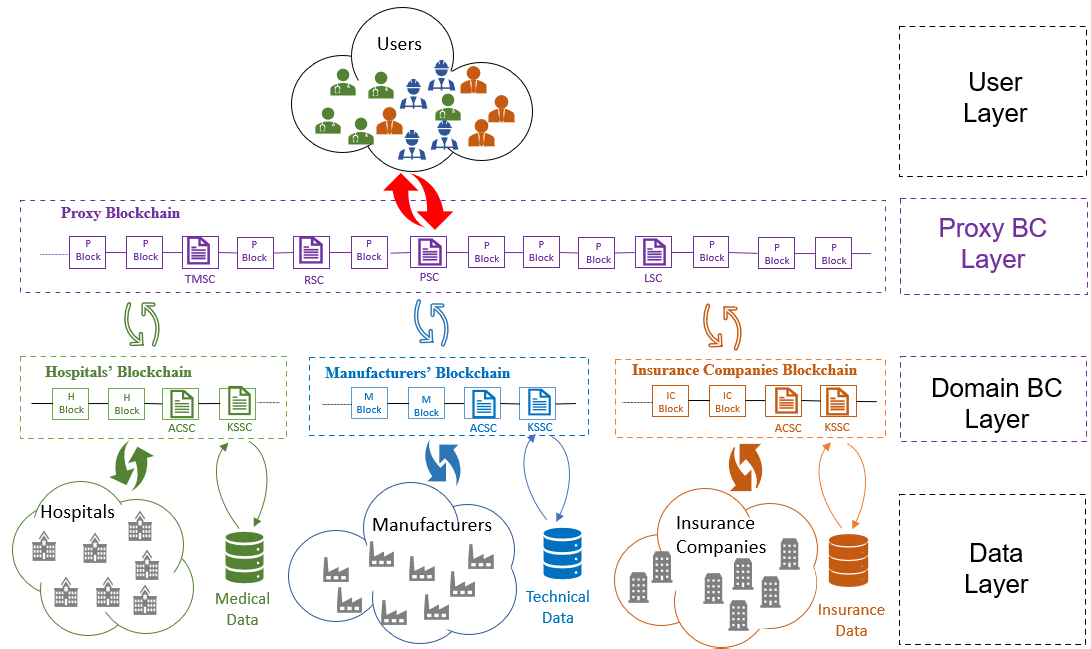
\includegraphics[height=2.6cm]{figures/fig1-architecture.png}};
  \end{tikzpicture}}
\hypersetup{pdftitle={HMBC end presentation: RQ1 complete, RQ2 partial (Team 17)}}

\begin{document}

% ================================================================ PART I: the paper (slides 1-3) and JANUS (slide 4)

% ---------------------------------------------------------------- 1. Title
\maketitle

% ---------------------------------------------------------------- 2. The paper (A): problem and architecture
\begin{frame}{The paper (1/2): the problem, and HMBC's architecture}
\begin{columns}[T,onlytextwidth]
\column{0.53\textwidth}
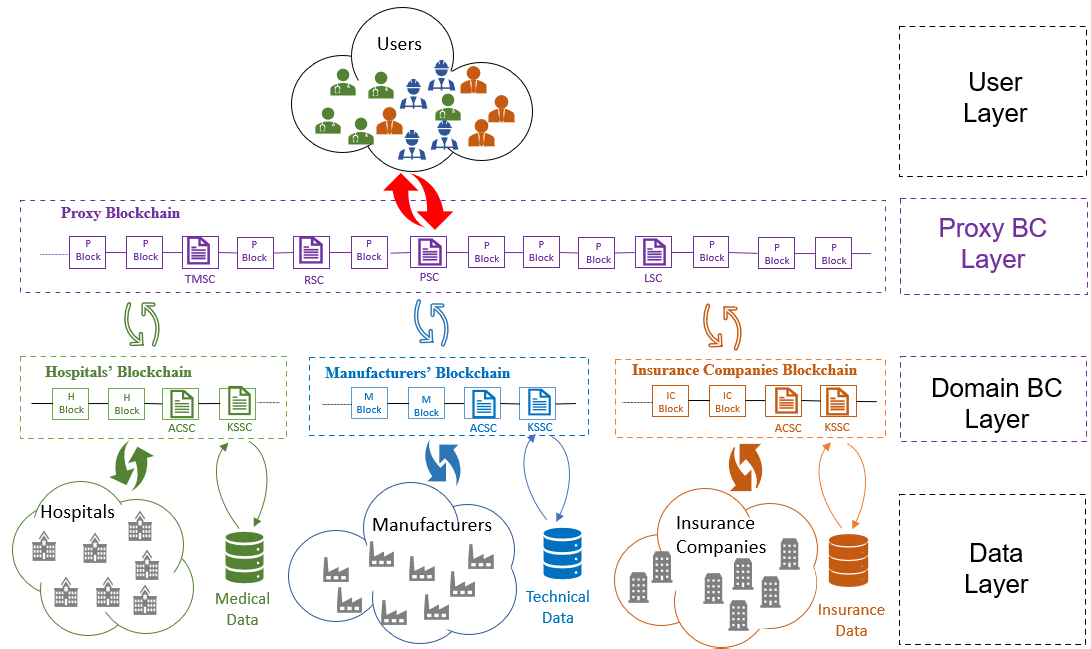
\includegraphics[width=\linewidth]{figures/fig1-architecture.png}\\[-0.1em]
\src{Paper Fig.~1 (CC BY 4.0)}\\[0.4em]
\centering
\resizebox{\linewidth}{!}{%

\begin{tikzpicture}[sc/.style={box, minimum height=0.5cm, text width=1.05cm, font=\tiny}]
  \node[font=\tiny\bfseries, text=pbc] at (-0.95,0) {PBC};
  \node[sc, draw=pbc, fill=pbc!10] at (0,0)    {\textbf{RSC}\\registration};
  \node[sc, draw=pbc, fill=pbc!10] at (1.2,0)  {\textbf{TMSC}\\trust lists};
  \node[sc, draw=pbc, fill=pbc!10] at (2.4,0)  {\textbf{PSC}\\entry point};
  \node[sc, draw=pbc, fill=pbc!10] at (3.6,0)  {\textbf{LSC}\\global log};
  \node[sc, draw=dbc, fill=dbc!12] at (5.0,0)  {\textbf{ACSC}\\access policy};
  \node[sc, draw=dbc, fill=dbc!12] at (6.2,0)  {\textbf{KSSC}\\key store};
  \node[font=\tiny\bfseries, text=dbc] at (7.15,0) {DBC};
\end{tikzpicture}}

\column{0.44\textwidth}
\scriptsize
\textbf{The problem.} Hospitals, device makers, insurers and researchers must share medical data, but \alert{they do not trust each other}, and each one manages its own users. A cloud makes sharing easy but needs a trusted operator; existing blockchains serve one domain.\\[0.3em]
\textbf{Running example:} an emergency doctor from Hospital~X needs a patient's history held at Hospital~Y, \emph{only while on duty}. The access must be revocable and logged.\\[0.3em]
\textbf{The actors}
\begin{itemize}\setlength{\itemsep}{1pt}
  \item \textbf{Users} (people and devices), each with one global ID (GID).
  \item \textbf{Stakeholders:} each runs its own CA and ABE key authority, and one node on each chain. Its CA admins publish trust lists.
  \item \textbf{\textcolor{pbc}{Proxy chain (PBC)}}, run by all: registration, trust lists (CERT, CRL, TempACL), the single entry point and the global log.
  \item \textbf{\textcolor{dbc}{Domain chains (DBC)}}, one per domain: access policy and key store. Users never talk to them.
  \item \textbf{Data owners} keep records off chain, ABE-encrypted.
\end{itemize}
\end{columns}
\note{Paper §I, §III (Fig. 1, Fig. 3/4); condensed from mid-eval slides 2-5.}
\end{frame}

% ---------------------------------------------------------------- 3. The paper (B): access overview + assumptions
\begin{frame}{The paper (2/2): how access works, and what it assumes}
\centering
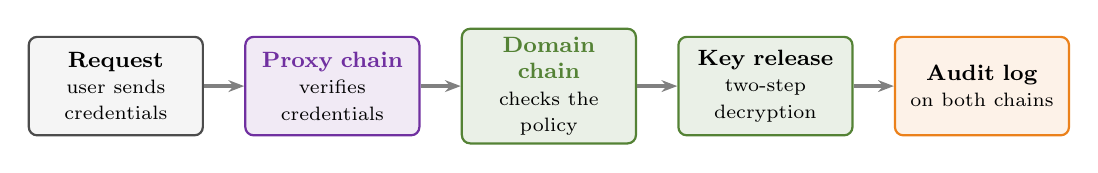
\begin{tikzpicture}[x=1cm, y=1cm,
    stg/.style={draw, thick, rounded corners=3pt, text width=2.0cm, minimum height=1.25cm, align=center, inner sep=3pt, font=\footnotesize, execute at begin node={\hyphenpenalty=10000\exhyphenpenalty=10000}},
    sub/.style={font=\scriptsize, text=datagray}]
  \node[stg, draw=black!70, fill=gray!8]  (a) at (0,0)    {\textbf{Request}\\{\scriptsize user sends credentials}};
  \node[stg, draw=pbc, fill=pbc!10]       (b) at (2.75,0) {\textbf{\textcolor{pbc}{Proxy chain}}\\{\scriptsize verifies credentials}};
  \node[stg, draw=dbc, fill=dbc!12]       (c) at (5.5,0)  {\textbf{\textcolor{dbc}{Domain chain}}\\{\scriptsize checks the policy}};
  \node[stg, draw=dbc, fill=dbc!12]       (d) at (8.25,0) {\textbf{Key release}\\{\scriptsize two-step decryption}};
  \node[stg, draw=accent, fill=accent!10] (e) at (11.0,0) {\textbf{Audit log}\\{\scriptsize on both chains}};
  \foreach \x/\y in {a/b, b/c, c/d, d/e} \draw[->, very thick, gray] (\x) -- (\y);
\end{tikzpicture}\\[0.15em]
\src{Overview, simplified from paper Fig.~6}

\vspace{0.6em}
\begin{columns}[T,onlytextwidth]
\column{0.48\textwidth}
\footnotesize\textbf{Key idea: split the decryption}
\begin{itemize}\scriptsize\setlength{\itemsep}{2pt}
  \item The key store (KSSC) keeps the temporal \emph{onDuty} key; the user holds the long-term \emph{Doctor} key. Neither decrypts alone.
  \item \textbf{Revocation is a list update:} ending a duty removes a TempACL entry; no key is re-issued.
\end{itemize}

\column{0.49\textwidth}
\begin{alertblock}{The paper's informal argument assumes}
\scriptsize isolation \,·\, an honest majority in every chain \,·\, secure crypto \,·\, uncompromised keys
\end{alertblock}
\scriptsize
\textbf{\textcolor{accent}{RQ1}}: what does the flow guarantee, and what depends on details it leaves open?\\[0.2em]
\textbf{\textcolor{pbc}{RQ2}}: what survives when the honest majority fails?
\end{columns}
\note{Paper Fig. 5 and 6, §III-E2, §V; mid-eval slides 6-8. Steps of Fig. 6: request and log record at the PSC/LSC; TMSC checks CERT, CRL, TempACL; ACSC checks the policy; KSSC does decryption step 1; ACSC logs on the DBC, LSC stores the record on the PBC; the user finishes decryption. The paper's prototype: 603 ms per access (Table 4).}
\end{frame}

% ---------------------------------------------------------------- 4. JANUS
\begin{frame}{JANUS: the authors' extension of HMBC}
\begin{columns}[T,onlytextwidth]
\column{0.41\textwidth}
\centering
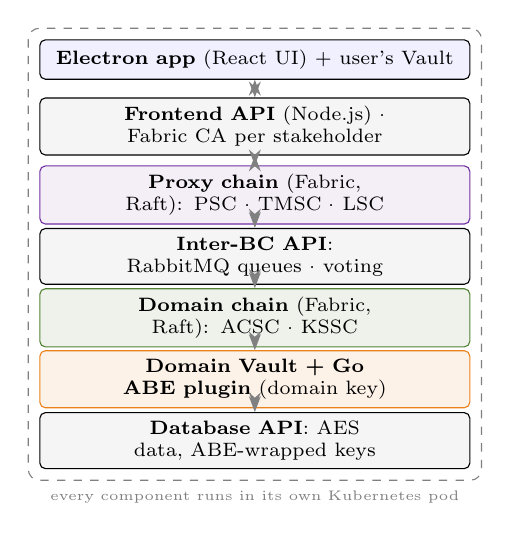
\begin{tikzpicture}[x=1cm, y=1cm, jl/.style={box, text width=5.25cm, minimum height=0.5cm}]
  \node[jl, fill=blue!6]                    (fe) at (0,0)     {\textbf{Electron app} (React UI) + user's Vault};
  \node[jl, fill=gray!8]                    (fa) at (0,-0.85) {\textbf{Frontend API} (Node.js) · Fabric CA per stakeholder};
  \node[jl, draw=pbc, fill=pbc!8]           (pc) at (0,-1.72) {\textbf{Proxy chain} (Fabric, Raft): PSC · TMSC · LSC};
  \node[jl, fill=gray!8]                    (ib) at (0,-2.5) {\textbf{Inter-BC API}: RabbitMQ queues · voting};
  \node[jl, draw=dbc, fill=dbc!10]          (dc) at (0,-3.28) {\textbf{Domain chain} (Fabric, Raft): ACSC · KSSC};
  \node[jl, draw=accent, fill=accent!10]    (va) at (0,-4.06)  {\textbf{Domain Vault + Go ABE plugin} (domain key)};
  \node[jl, fill=gray!8]                    (db) at (0,-4.84) {\textbf{Database API}: AES data, ABE-wrapped keys};
  \foreach \a/\b in {fe/fa,fa/pc,pc/ib,ib/dc,dc/va,va/db} \draw[<->, thick, gray] (\a.south) -- (\b.north);
  \node[draw, dashed, gray, rounded corners, fit=(fe)(db), inner sep=4pt] (k8s) {};
  \node[font=\tiny, text=gray, anchor=north] at (k8s.south) {every component runs in its own Kubernetes pod};
\end{tikzpicture}\\[0.1em]
\src{Simplified from JANUS Fig.~5}

\column{0.56\textwidth}
\footnotesize
\textbf{JANUS} extends HMBC. It is by HMBC's authors (Malamas, Kotzanikolaou, Burmester) with CENSUS S.A., \emph{Applied Sciences} 13(1):566, 2023.\\[0.4em]
\textbf{Main extensions}
\begin{itemize}\scriptsize\setlength{\itemsep}{2pt}
  \item \textbf{A formal access model (HMBAC):} attribute verification on the PBC; authorisation and decryption on the DBC.
  \item \textbf{An open-source system:} Hyperledger Fabric 2.4 + Raft, JavaScript contracts, Kubernetes pods.
  \item \textbf{Single access point enforced by crypto:} a \emph{domain key} that only the KSSC can derive (in Vault) is ANDed into every policy.
  \item \textbf{Hybrid encryption:} AES for records, MA-ABE only for the AES keys.
  \item \textbf{Engineering:} RabbitMQ queues with throttling; voting for domains, stakeholders and policies.
  \item \textbf{Evaluation:} attack trees; 2--300 concurrent requests, no failed requests.
\end{itemize}
\vspace{0.3em}
\scriptsize\textbf{\textcolor{accent}{Left open:}} Raft tolerates crashes only; Byzantine tolerance is named as future work.\\[0.3em]
{\color{datagray}Related work only: we implement HMBC and use no JANUS code.}
\end{columns}
\note{JANUS = Malamas, Palaiologos, Kotzanikolaou, Burmester, Glynos, Appl. Sci. 13(1):566, 2023, doi 10.3390/app13010566. Facts from mid-eval slides 9-10 (origin/slides d292576, hmbc-presentation.tex lines 331-386).}
\end{frame}

% ---------------------------------------------------------------- 5. Our research questions
\begin{frame}{What we set out to answer: two research questions}
\centering
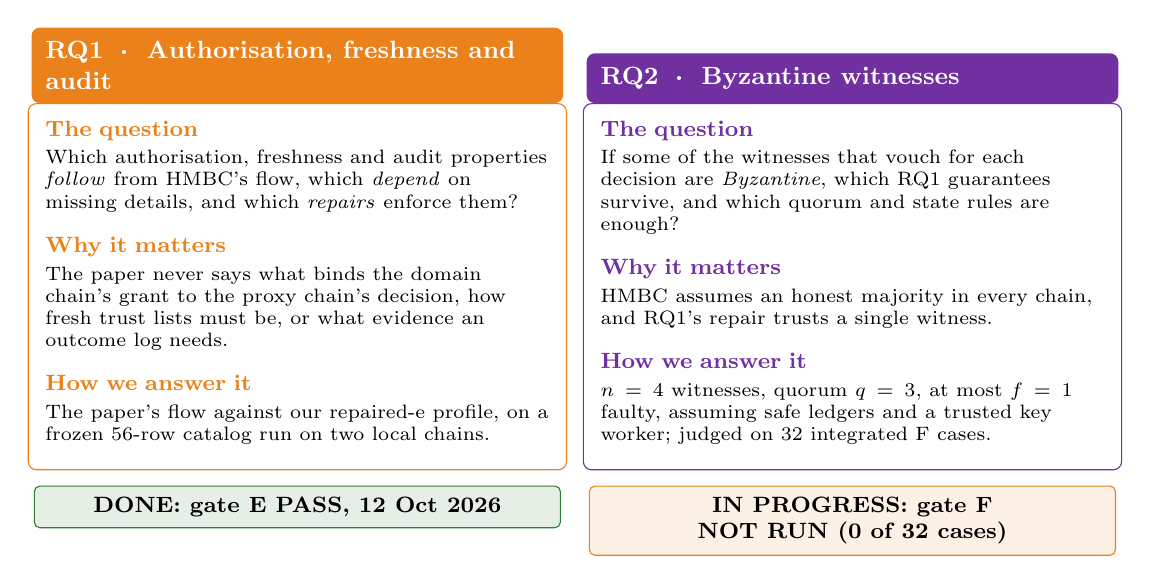
\begin{tikzpicture}[x=1cm, y=1cm,
    card/.style={text width=6.4cm, align=left, inner sep=6pt, font=\scriptsize, anchor=north, execute at begin node={\hyphenpenalty=10000\exhyphenpenalty=10000}},
    head/.style={rounded corners=3pt, text width=6.4cm, inner sep=5pt, font=\small\bfseries, text=white, anchor=south},
    stn/.style={rounded corners=2pt, text width=6.4cm, inner sep=4pt, font=\footnotesize\bfseries, align=center, anchor=north}]
  \node[card] (c1) at (0,0) {%
    {\footnotesize\color{accent}\textbf{The question}}\\[2pt]
    Which authorisation, freshness and audit properties \emph{follow} from HMBC's flow, which \emph{depend} on missing details, and which \emph{repairs} enforce them?\\[8pt]
    {\footnotesize\color{accent}\textbf{Why it matters}}\\[2pt]
    The paper never says what binds the domain chain's grant to the proxy chain's decision, how fresh trust lists must be, or what evidence an outcome log needs.\\[8pt]
    {\footnotesize\color{accent}\textbf{How we answer it}}\\[2pt]
    The paper's flow against our repaired-e profile, on a frozen 56-row catalog run on two local chains.};
  \node[head, fill=accent] at (0,0) {RQ1 \;·\; Authorisation, freshness and audit};
  \node[card] (c2) at (7.05,0) {%
    {\footnotesize\color{pbc}\textbf{The question}}\\[2pt]
    If some of the witnesses that vouch for each decision are \emph{Byzantine}, which RQ1 guarantees survive, and which quorum and state rules are enough?\\[8pt]
    {\footnotesize\color{pbc}\textbf{Why it matters}}\\[2pt]
    HMBC assumes an honest majority in every chain, and RQ1's repair trusts a single witness.\\[8pt]
    {\footnotesize\color{pbc}\textbf{How we answer it}}\\[2pt]
    $n = 4$ witnesses, quorum $q = 3$, at most $f = 1$ faulty, assuming safe ledgers and a trusted key worker; judged on 32 integrated F cases.};
  \node[head, fill=pbc] at (7.05,0) {RQ2 \;·\; Byzantine witnesses};
  \draw[accent, rounded corners=3pt] (c1.north west) rectangle ($(c1.north east)+(0,-4.65)$);
  \draw[pbc, rounded corners=3pt] (c2.north west) rectangle ($(c2.north east)+(0,-4.65)$);
  \node[stn, draw=okgreen, fill=okgreen!12] at (0,-4.85) {DONE: gate E PASS, 12 Oct 2026};
  \node[stn, draw=accent, fill=accent!12] at (7.05,-4.85) {IN PROGRESS: gate F NOT RUN (0 of 32 cases)};
\end{tikzpicture}
\note{RQ wording: SPEC.md §1, RQ1-E.md §1, RQ2-F-DRAFT.md §1. Gaps: RQ1-E.md §0. Assumptions: paper §V. One trusted witness: RQ1-E.md §15. Catalog: RQ1-E.md §3.3. Fault model: RQ2-F-DRAFT.md §1; 32 cases: plan-draft.json.}
\end{frame}

% ================================================================ PART II: RQ1 (slides 6-14), adapted from mid-eval slides 15-22
% Source of every number below: evaluation/reports/RQ1-E.md (69dabfba..), communication/GATES.md (E section),
% interfaces/v1/source-map.csv and assumptions.csv, and the owner window measurements A1-0046 / A2-0026.

% ---------------------------------------------------------------- 6. RQ1 question and gaps
\begin{frame}{RQ1: the question, and what HMBC's flow leaves unspecified}
\begin{center}
\vspace{-0.3em}
\scriptsize\itshape Which authorisation, trust-freshness and audit properties \emph{follow} from HMBC's access flow, which \emph{depend} on details the paper leaves out, and which explicit \emph{repairs} enforce them?
\end{center}
\vspace{-0.4em}
\begin{columns}[T,onlytextwidth]
\column{0.50\textwidth}
\centering
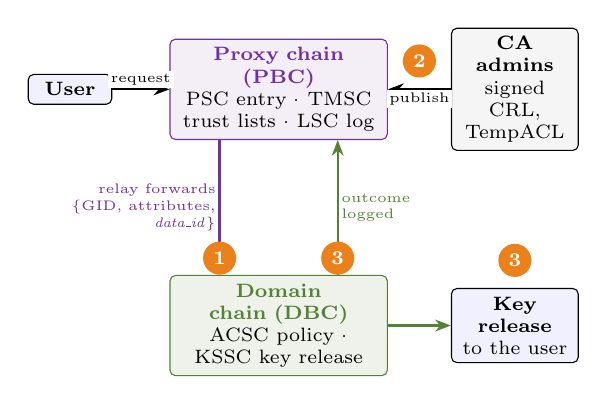
\begin{tikzpicture}[x=1cm, y=1cm,
    gap/.style={circle, fill=accent, text=white, font=\scriptsize\bfseries, inner sep=1.2pt, minimum size=0.42cm}]
  \node[box, fill=blue!6, text width=0.85cm] (u) at (0,0) {\textbf{User}};
  \node[box, draw=pbc, fill=pbc!8, text width=2.55cm, minimum height=1.05cm] (pbc) at (2.65,0)
       {\textbf{\textcolor{pbc}{Proxy chain (PBC)}}\\PSC entry · TMSC trust lists · LSC log};
  \node[box, fill=gray!8, text width=1.4cm] (ca) at (5.65,0) {\textbf{CA admins}\\signed CRL, TempACL};
  \node[box, draw=dbc, fill=dbc!10, text width=2.55cm, minimum height=1.05cm] (dbc) at (2.65,-3.0)
       {\textbf{\textcolor{dbc}{Domain chain (DBC)}}\\ACSC policy · KSSC key release};
  \node[box, fill=blue!6, text width=1.4cm] (rel) at (5.65,-3.0) {\textbf{Key release}\\to the user};
  \draw[->, thick] (u) -- node[lbl, above, font=\tiny] {request} (pbc);
  \draw[->, thick] (ca) -- node[lbl, below, font=\tiny] {publish} (pbc);
  \draw[->, thick, pbc] ($(pbc.south)+(-0.75,0)$) -- node[lbl, left, align=right, text width=1.9cm, font=\tiny] {relay forwards\\$\{$GID, attributes,\\\textit{data\_id}$\}$} ($(dbc.north)+(-0.75,0)$);
  \draw[->, thick, dbc] ($(dbc.north)+(0.75,0)$) -- node[lbl, right, align=left, font=\tiny] {outcome\\logged} ($(pbc.south)+(0.75,0)$);
  \draw[->, thick, dbc] (dbc) -- (rel);
  \node[gap] at ($(pbc.south)+(-0.75,-1.5)$) {1};
  \node[gap] at ($(pbc.east)!0.5!(ca.west)+(0,0.36)$) {2};
  \node[gap] at ($(pbc.south)+(0.75,-1.5)$) {3};
  \node[gap] at ($(rel.north)+(0,0.35)$) {3};
\end{tikzpicture}\\[0.2em]
\src{Simplified from paper Fig.~6; circles mark the gaps}

\column{0.47\textwidth}
\footnotesize
\renewcommand{\arraystretch}{1.25}
\begin{tabular}{@{}c L{0.88\linewidth}@{}}
\gapn{1} & \textbf{RQ1-01 decision provenance.} The DBC sees a tuple, not the PBC's decision. Nothing says \emph{who} it is for, \emph{which chain} it targets, \emph{when} it expires, or that it is \emph{new}. \\
\gapn{2} & \textbf{RQ1-02 trust-anchor freshness.} Lists are ``the latest'', with no version or expiry. Nothing says \emph{when} a revocation must reach the DBC. \\
\gapn{3} & \textbf{RQ1-03 audit correspondence.} An outcome can be logged without DBC evidence. The paper is silent on a crash between key release and logging. \\
\end{tabular}
\end{columns}
\note{Source map: 37 paper passages (S01-S37) and 41 recorded completions (A01-A41) in interfaces/v1. Gap 1 is A02/A14/A19/A25, gap 2 A09/A17/A20/A22, gap 3 A03/A11/A12/A26.}
\end{frame}

% ---------------------------------------------------------------- 7. RQ1 method
\begin{frame}{RQ1 method: the paper and our repair on one frozen catalog}
\begin{columns}[T,onlytextwidth]
\column{0.40\textwidth}
\footnotesize\textbf{Four profiles of the same six contracts}\\[0.3em]
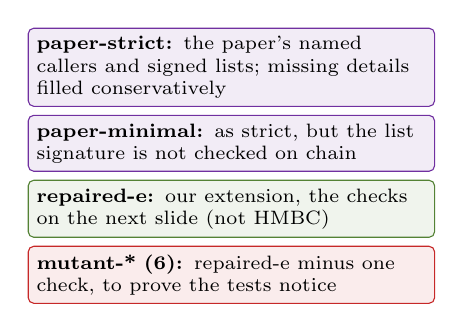
\begin{tikzpicture}[x=1cm, y=1cm, every node/.append style={execute at begin node={\hyphenpenalty=10000\exhyphenpenalty=10000}}]
  \node[prof=pbc, anchor=north west] (a) at (0,0) {\textbf{paper-strict:} the paper's named callers and signed lists; missing details filled conservatively};
  \node[prof=pbc, anchor=north west] (b) at ($(a.south west)+(0,-0.1)$) {\textbf{paper-minimal:} as strict, but the list signature is not checked on chain};
  \node[prof=dbc, anchor=north west] (c) at ($(b.south west)+(0,-0.1)$) {\textbf{repaired-e:} our extension, the checks on the next slide (not HMBC)};
  \node[prof=badred, anchor=north west] (d) at ($(c.south west)+(0,-0.1)$) {\textbf{mutant-* (6):} repaired-e minus one check, to prove the tests notice};
\end{tikzpicture}

\vspace{0.4em}
\textbf{Each row gets one class}\\[0.1em]
\scriptsize
\renewcommand{\arraystretch}{1.15}
\begin{tabular}{@{}l L{0.60\linewidth}@{}}
\cSup & follows from the paper (as reconstructed) \\
\cGap & depends on a detail the paper leaves open \\
\cRep & our repair enforces it \\
\cBlk & cannot be decided from the paper \\
\end{tabular}

\column{0.57\textwidth}
\footnotesize\textbf{How each result is produced}\\[0.3em]
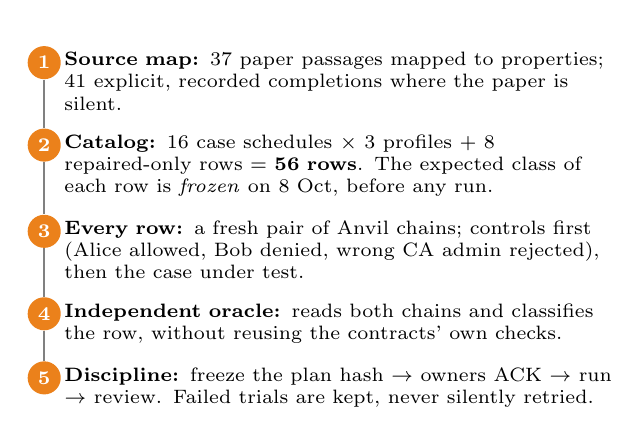
\begin{tikzpicture}[x=1cm, y=1cm,
    num/.style={circle, fill=accent, text=white, font=\scriptsize\bfseries, inner sep=1pt, minimum size=0.42cm},
    st/.style={text width=7.0cm, align=left, font=\scriptsize, anchor=north west, inner sep=0pt, execute at begin node={\hyphenpenalty=10000\exhyphenpenalty=10000}}]
  \node[inner sep=0pt, minimum size=0pt] (t-1) at (0.4,0.3) {};
  \foreach \i/\t in {
      0/{\textbf{Source map:} 37 paper passages mapped to properties; 41 explicit, recorded completions where the paper is silent.},
      1/{\textbf{Catalog:} 16 case schedules $\times$ 3 profiles + 8 repaired-only rows = \textbf{56 rows}. The expected class of each row is \emph{frozen} on 8 Oct, before any run.},
      2/{\textbf{Every row:} a fresh pair of Anvil chains; controls first (Alice allowed, Bob denied, wrong CA admin rejected), then the case under test.},
      3/{\textbf{Independent oracle:} reads both chains and classifies the row, without reusing the contracts' own checks.},
      4/{\textbf{Discipline:} freeze the plan hash $\rightarrow$ owners ACK $\rightarrow$ run $\rightarrow$ review. Failed trials are kept, never silently retried.}} {
    \pgfmathtruncatemacro{\prev}{\i-1}
    \node[st] (t\i) at ($(t\prev.south west)+(0,-0.3)$) {\t};
    \node[num, anchor=north] (n\i) at ($(t\i.north west)+(-0.25,0.08)$) {\the\numexpr\i+1\relax};
  }
  \foreach \i [evaluate=\i as \j using int(\i+1)] in {0,...,3} \draw[gray, thick] (n\i) -- (n\j);
\end{tikzpicture}
\end{columns}
\note{Catalog: interfaces/v1/scenarios/e0_cases.json (48 rows = 16 schedules x 3 profiles) plus e0_supplement_cases.json (8 repaired-e rows). Positive controls: e_positive.json. Interface v1 FREEZE f700292e.. on 2026-10-08.}
\end{frame}

% ---------------------------------------------------------------- 8. What repaired-e adds
\begin{frame}{RQ1: what we built, the repaired-e profile}
\centering
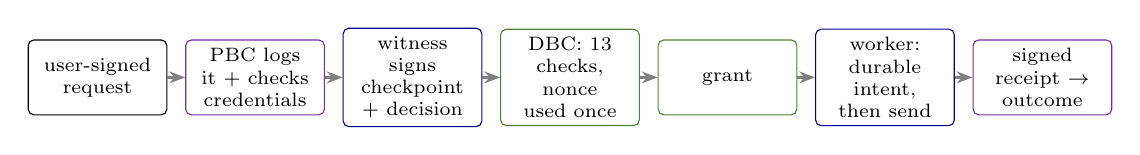
\begin{tikzpicture}[x=1cm, y=1cm, st/.style={box, text width=1.55cm, minimum height=0.95cm, fill=white}]
  \foreach \i/\t/\col in {0/{user-signed request}/black, 1/{PBC logs it + checks credentials}/pbc, 2/{witness signs checkpoint + decision}/blue!60!black, 3/{DBC: 13 checks, nonce used once}/dbc, 4/{grant}/dbc, 5/{worker: durable intent, then send}/blue!60!black, 6/{signed receipt $\to$ outcome}/pbc} {
    \node[st, draw=\col] (s\i) at (\i*2.0,0) {\t};
  }
  \foreach \i [evaluate=\i as \j using int(\i+1)] in {0,...,5} \draw[->, thick, gray] (s\i) -- (s\j);
\end{tikzpicture}

\vspace{0.5em}
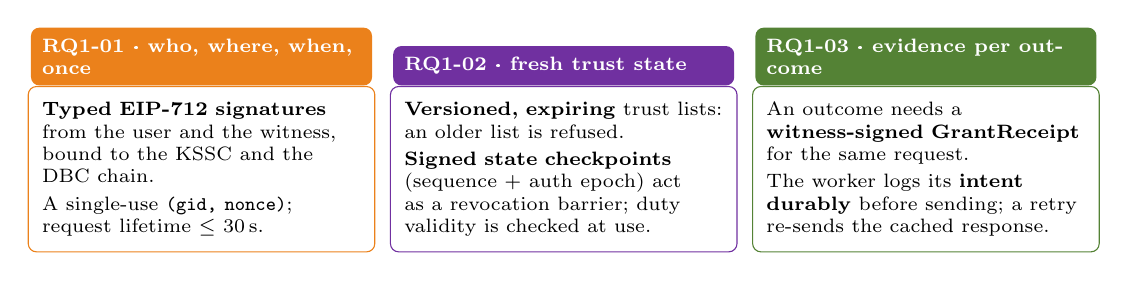
\begin{tikzpicture}[x=1cm, y=1cm, cw/.style={text width=4.05cm, minimum height=2.1cm, execute at begin node={\hyphenpenalty=10000\exhyphenpenalty=10000}}, hw/.style={text width=4.05cm, font=\scriptsize\bfseries}]
  \node[pcard=accent, cw] at (0,0) {%
    \textbf{Typed EIP-712 signatures} from the user and the witness, bound to the KSSC and the DBC chain.\\[2pt]
    A single-use \texttt{(gid, nonce)}; request lifetime $\le$ 30\,s.};
  \node[phead=accent, hw] at (0,0) {RQ1-01 · who, where, when, once};
  \node[pcard=pbc, cw] at (4.6,0) {%
    \textbf{Versioned, expiring} trust lists: an older list is refused.\\[2pt]
    \textbf{Signed state checkpoints} (sequence + auth epoch) act as a revocation barrier; duty validity is checked at use.};
  \node[phead=pbc, hw] at (4.6,0) {RQ1-02 · fresh trust state};
  \node[pcard=dbc, cw] at (9.2,0) {%
    An outcome needs a \textbf{witness-signed GrantReceipt} for the same request.\\[2pt]
    The worker logs its \textbf{intent durably} before sending; a retry re-sends the cached response.};
  \node[phead=dbc, hw] at (9.2,0) {RQ1-03 · evidence per outcome};
\end{tikzpicture}

\vspace{0.45em}
{\scriptsize\textbf{DecisionVerifier on the DBC: 13 checks in a fixed order} (colours as above; step 12 is reserved and not used here)}\\[0.25em]
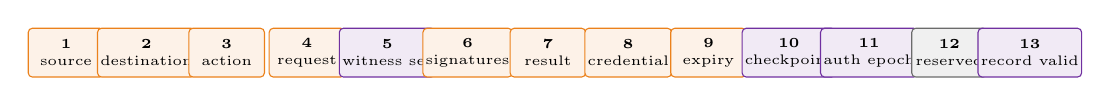
\begin{tikzpicture}[x=1cm, y=1cm]
  \foreach \i/\t/\col in {1/source/accent, 2/destination/accent, 3/action/accent, 4/request/accent, 5/witness set/pbc, 6/signatures/accent, 7/result/accent, 8/credential/accent, 9/expiry/accent, 10/checkpoint/pbc, 11/auth epoch/pbc, 12/reserved/datagray, 13/record valid/pbc} {
    \node[dv=\col, minimum width=0.96cm] at (\i*1.02,0) {\textbf{\i}\\\t};
  }
\end{tikzpicture}\\[0.1em]
{\scriptsize Several defects always give the same error code; contracts hold no secrets; in RQ1 the witness is \textbf{one trusted party}.}
\note{repaired-e is a project extension, not HMBC. Six mutants each remove one check: destination binding (1), state barrier (2), record freshness (4), nonce (8), version monotonicity (16), receipt binding (32).}
\end{frame}

% ---------------------------------------------------------------- 9. E01 results
\begin{frame}{RQ1 results, gap 1: decision provenance and replay \;\evl{I}}
\scriptsize
\renewcommand{\arraystretch}{1.12}
\begin{tabular}{@{}L{0.27\textwidth} L{0.33\textwidth} L{0.37\textwidth}@{}}
\toprule
\textbf{The relay\ldots} & \textbf{paper-strict / paper-minimal} & \textbf{repaired-e} \\
\midrule
replays an identical accepted request & \cSup\ rejected: \code{REPLAY}\textsuperscript{$*$} & \cRep\ rejected: \code{REPLAY} \\
swaps the subject (GID) & \cGap\ granted; response goes to the swapped subject & \cRep\ \code{WRONG\_SUBJECT}, step 4 \\
forges a tuple with no PBC request & \cGap\ granted & \cRep\ \code{BAD\_SIGNATURE}, step 6 \\
replays it under a new reference & \cGap\ a second grant & \cRep\ \code{REPLAY}: grant already exists \\
reuses a nonce on a different request & -- (the paper has no nonce) & \cRep\ \code{REPLAY}: nonce already used \\
delivers deployment B's tuple to A & \cGap\ A grants it & \cRep\ \code{WRONG\_DESTINATION}, step 1 \\
delivers it exactly at the request's expiry & \cGap\ granted at that instant & \cRep\ \code{EXPIRED}, step 9 (at equality) \\
\bottomrule
\end{tabular}\\[0.15em]
{\scriptsize\color{datagray}\textbf{Evidence labels:} [I] integrated evaluator run \,·\, [R] owners' cross-run \,·\, [U] unit or offline test \,·\, [F] formal model}

\vspace{0.35em}
\begin{columns}[T,onlytextwidth]
\column{0.62\textwidth}
\begin{alertblock}{What it means}
\scriptsize In the paper profiles the DBC grants \emph{any} well-formed tuple the configured relay forwards. Repaired-e rejects each attack at a named verifier step, and Alice's legitimate access still succeeds in every row.
\end{alertblock}
\column{0.35\textwidth}
\scriptsize\color{datagray}
\textsuperscript{$*$}Only because our grant id is deterministic (a recorded completion), not because the paper has a nonce.\\[3pt]
The relay attacks use a misbehaving relay, which HMBC's isolation assumption excludes.\\[3pt]
\src{RQ1-E.md §0, §7; gate rows 10--22, 51--56}
\end{columns}
\end{frame}

% ---------------------------------------------------------------- 10. E02 results + window
\begin{frame}{RQ1 results, gap 2: trust-anchor freshness and the revocation window}
\begin{columns}[T,onlytextwidth]
\column{0.56\textwidth}
\scriptsize
\renewcommand{\arraystretch}{1.3}
\begin{tabular}{@{}L{0.30\linewidth} L{0.32\linewidth} L{0.32\linewidth}@{}}
\toprule
\textbf{Case} \evl{I} & \textbf{paper profiles} & \textbf{repaired-e} \\
\midrule
CA admin updates another issuer's list & \cSup\ \code{UNAUTHORIZED\_CALLER} (baseline, not a repair) & \cSup\ same \\
an older signed CRL is re-installed & \cGap\ accepted: a \textbf{revoked credential is un-revoked} & \cRep\ \code{STALE\_ANCHOR} \\
revoked; decision used \emph{before} the DBC sees a new checkpoint & \cGap\ accepted & \cRep\ accepted on purpose, inside the bounded window \\
revoked; decision used \emph{after} it & \cGap\ still accepted: there is no barrier & \cRep\ \code{STALE\_STATE} \\
duty ended at delivery & \cGap\ granted at that instant & \cRep\ \code{EXPIRED} (step 13) \\
\bottomrule
\end{tabular}\\[0.3em]
\src{RQ1-E.md §0, §8; gate rows 36--50}

\column{0.41\textwidth}
\centering
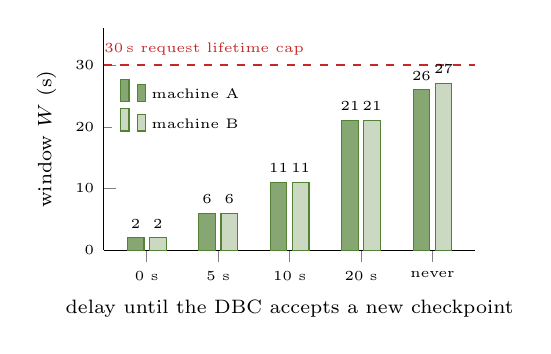
\begin{tikzpicture}
\begin{axis}[
    ybar, bar width=6pt, width=6.3cm, height=4.4cm,
    ymin=0, ymax=36, axis x line*=bottom, axis y line*=left,
    symbolic x coords={0 s,5 s,10 s,20 s,never},
    xtick=data, enlarge x limits=0.15,
    xlabel={delay until the DBC accepts a new checkpoint},
    ylabel={window $W$ (s)},
    tick label style={font=\tiny}, label style={font=\scriptsize},
    nodes near coords, nodes near coords style={font=\tiny},
    legend style={font=\tiny, at={(0.02,0.80)}, anchor=north west, draw=none, fill=white},
    legend cell align=left,
  ]
  \addplot[fill=dbc!70, draw=dbc] coordinates {(0 s,2) (5 s,6) (10 s,11) (20 s,21) (never,26)};
  \addplot[fill=dbc!30, draw=dbc] coordinates {(0 s,2) (5 s,6) (10 s,11) (20 s,21) (never,27)};
  \draw[dashed, badred, thick] (rel axis cs:0,0.833) -- (rel axis cs:1,0.833) node[pos=0.27, above, font=\tiny, text=badred] {30\,s request lifetime cap};
  \legend{machine A, machine B}
\end{axis}
\end{tikzpicture}\\
\scriptsize
\textbf{repaired-e:} $W = \min(\text{checkpoint delay}, \text{lifetime left}) \le 30$\,s\\[1pt]
\textbf{paper-strict:} no bound; still grantable 65\,s later\\[2pt]
\src{owner measurement \evl{R}, 1 trial per delay; not the gate run (A1-0046, A2-0026)}
\end{columns}
\end{frame}

% ---------------------------------------------------------------- 11. E03 results
\begin{frame}{RQ1 results, gap 3: audit correspondence and crash recovery \;\evl{I}}
\begin{columns}[T,onlytextwidth]
\column{0.60\textwidth}
\scriptsize
\renewcommand{\arraystretch}{1.3}
\begin{tabular}{@{}L{0.30\linewidth} L{0.30\linewidth} L{0.34\linewidth}@{}}
\toprule
\textbf{Case} & \textbf{paper profiles} & \textbf{repaired-e} \\
\midrule
same outcome reported twice & \cSup\ \code{REPLAY} & \cRep\ \code{REPLAY} \\
relay drops the outcome & \cSup\ request stays PENDING, visibly & \cRep\ same, plus durable worker evidence \\
outcome fabricated, no grant exists & \cGap\ recorded & \cRep\ \code{WRONG\_PROFILE}: needs a receipt \\
receipt names another request, GID or record & -- (no receipts) & \cRep\ \code{WRONG\_SUBJECT}, nothing recorded \\
worker crashes after intent / after send & \cBlk\ the paper is silent on durability & \cRep\ cached response re-sent: one grant, one outcome \\
\bottomrule
\end{tabular}

\column{0.37\textwidth}
\centering
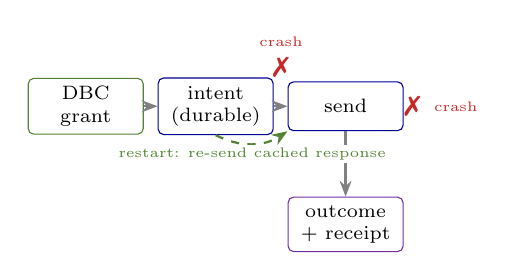
\begin{tikzpicture}[x=1cm, y=1cm, ev/.style={box, text width=1.25cm, minimum height=0.62cm, fill=white}]
  \node[ev, draw=dbc] (g) at (0,0) {DBC grant};
  \node[ev, draw=blue!60!black] (i) at (1.65,0) {intent (durable)};
  \node[ev, draw=blue!60!black] (s) at (3.3,0) {send};
  \node[ev, draw=pbc] (o) at (3.3,-1.5) {outcome + receipt};
  \draw[->, thick, gray] (g) -- (i);
  \draw[->, thick, gray] (i) -- (s);
  \draw[->, thick, gray] (s) -- (o);
  \node[text=badred, font=\bfseries] at (2.48,0.5) {\ding{55}};
  \node[text=badred, font=\bfseries] at (4.15,0.0) {\ding{55}};
  \node[font=\tiny, text=badred] at (2.48,0.82) {crash};
  \node[font=\tiny, text=badred, anchor=west] at (4.3,0.0) {crash};
  \draw[->, thick, dbc, dashed] (i.south) to[bend right=30] node[lbl, below, font=\tiny, text=dbc] {restart: re-send cached response} (s.south west);
\end{tikzpicture}\\[0.4em]
\begin{itemize}\scriptsize
  \item Before the grant expires: the \emph{same} response again, no second capability.
  \item After it expires: \code{EXPIRED}, nothing changes.
  \item A grant is permission to release, \textbf{not proof of delivery}: delivery stays ``unknown'', and we report it that way.
\end{itemize}
\end{columns}

\vspace{0.4em}
\raggedright\scriptsize\color{datagray}
The four paper crash rows are recorded as ``BLOCKED / decided SPEC\_GAP, unproved'': never a pass, never a finding. Crash points are logical process deaths, not power loss. The receipt-substitution rows use a deliberately deviating test witness. \src{RQ1-E.md §9; gate rows 1--9, 23--35}
\end{frame}

% ---------------------------------------------------------------- 12. Mutants + ProVerif
\begin{frame}{RQ1: are the checks real? Mutants and a formal model}
\begin{columns}[T,onlytextwidth]
\column{0.53\textwidth}
\footnotesize\textbf{Remove one check, and something must fail} \evl{U}\\[0.3em]
\scriptsize
\renewcommand{\arraystretch}{1.22}
\begin{tabular}{@{}L{0.26\linewidth} L{0.29\linewidth} L{0.39\linewidth}@{}}
\toprule
\textbf{Mutant} & \textbf{Ledger test that fails} & \textbf{Gate row that hits the guard} \\
\midrule
no nonce & nonce reuse across requests & same nonce: \code{REPLAY} \\
no receipt binding & receipt field swap & receipt $\times$3: \code{WRONG\_SUBJECT} \\
no state barrier & revocation barrier & post-barrier: \code{STALE\_STATE} \\
no record freshness & duty ended at delivery & expired duty: \code{EXPIRED} \\
no version order & stale CRL / TempACL replay & rollback: \code{STALE\_ANCHOR} \\
no destination binding & request field swap; ProVerif & -- (step 1 fires first) \\
\bottomrule
\end{tabular}\\[0.4em]
\scriptsize All six are detected by their expected ledger tests; 8 gate rows hit exactly the guard a mutant removes.\\[0.2em]
\src{RQ1-E.md §12}

\column{0.44\textwidth}
\footnotesize\textbf{ProVerif: does each grant match the approvals?} \evl{F}\\[0.3em]
\centering
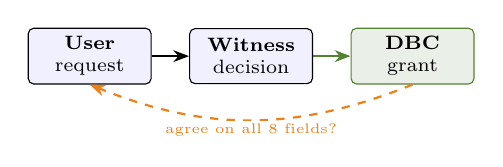
\begin{tikzpicture}[x=1cm, y=1cm, ev/.style={box, text width=1.35cm, minimum height=0.7cm}]
  \node[ev, fill=blue!6] (u) at (0,0) {\textbf{User}\\request};
  \node[ev, fill=blue!6] (w) at (2.05,0) {\textbf{Witness}\\decision};
  \node[ev, draw=dbc, fill=dbc!12] (g) at (4.1,0) {\textbf{DBC}\\grant};
  \draw[->, thick] (u) -- (w);
  \draw[->, thick, dbc] (w) -- (g);
  \draw[->, thick, accent, dashed] (g.south) to[bend left=22] node[lbl, below, text=accent, font=\tiny] {agree on all 8 fields?} (u.south);
\end{tikzpicture}\\[0.2em]
\scriptsize
\renewcommand{\arraystretch}{1.15}
\begin{tabular}{@{}L{0.44\linewidth} L{0.22\linewidth} L{0.26\linewidth}@{}}
\toprule
\textbf{Query} & \textbf{repaired} & \textbf{mutant} \\
\midrule
grant agrees with user + witness on all 8 fields & \textcolor{okgreen}{\textbf{true}} & \textcolor{badred}{\textbf{false}}: attack trace \\
other 7 fields agree & \textcolor{okgreen}{true} & \textcolor{okgreen}{true} \\
legitimate grant reachable & \textcolor{okgreen}{yes} & \textcolor{okgreen}{yes} \\
policy-denied grant & \textcolor{okgreen}{unreachable} & \textcolor{okgreen}{unreachable} \\
\bottomrule
\end{tabular}\\[0.3em]
\raggedright\scriptsize\color{datagray} Symbolic model (perfect signatures, one honest user and witness); no replay, expiry or revocation. \src{RQ1-E.md §11}
\end{columns}
\end{frame}

% ---------------------------------------------------------------- 13. Gate E
\begin{frame}{RQ1 gate E: one command, 56 rows, a recorded verdict}
\begin{columns}[T,onlytextwidth]
\column{0.56\textwidth}
\centering
\footnotesize\textbf{Every catalog row, coloured by its result} \evl{I}\\[0.4em]
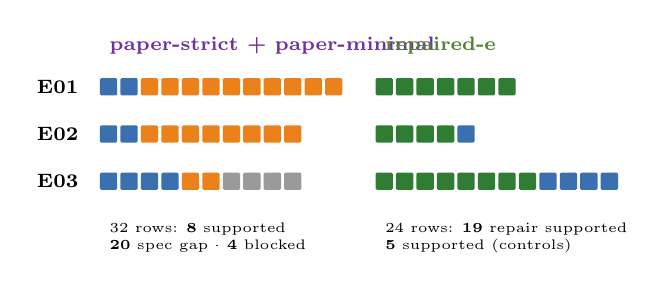
\begin{tikzpicture}[x=1cm, y=1cm]
  \node[font=\scriptsize\bfseries, text=pbc, anchor=south west] at (0.85,0.4) {paper-strict + paper-minimal};
  \node[font=\scriptsize\bfseries, text=dbc, anchor=south west] at (4.35,0.4) {repaired-e};
  \node[font=\scriptsize\bfseries, anchor=east] at (0.7,0.11)  {E01};
  \node[font=\scriptsize\bfseries, anchor=east] at (0.7,-0.49) {E02};
  \node[font=\scriptsize\bfseries, anchor=east] at (0.7,-1.09) {E03};
  \wcells{0.85}{0}{0}{2}{clsup}  \wcells{0.85}{2}{0}{10}{clgap}
  \wcells{4.35}{0}{0}{7}{clrep}
  \wcells{0.85}{0}{-0.6}{2}{clsup}  \wcells{0.85}{2}{-0.6}{8}{clgap}
  \wcells{4.35}{0}{-0.6}{4}{clrep}   \wcells{4.35}{4}{-0.6}{1}{clsup}
  \wcells{0.85}{0}{-1.2}{4}{clsup}  \wcells{0.85}{4}{-1.2}{2}{clgap}  \wcells{0.85}{6}{-1.2}{4}{clblk}
  \wcells{4.35}{0}{-1.2}{8}{clrep}   \wcells{4.35}{8}{-1.2}{4}{clsup}
  \node[font=\tiny, anchor=north west, align=left] at (0.85,-1.5) {32 rows: \textbf{8} supported\\\textbf{20} spec gap · \textbf{4} blocked};
  \node[font=\tiny, anchor=north west, align=left] at (4.35,-1.5) {24 rows: \textbf{19} repair supported\\\textbf{5} supported (controls)};
\end{tikzpicture}\\[0.5em]
\scriptsize
\cSup\ \ \cGap\ \ \cRep\ \ \cBlk\\[0.5em]
\raggedright\scriptsize Every gap in the paper profiles has a repaired-e row with an explicit check. In all 56 rows the observed class and error code equal the \textbf{frozen} expectation: 0 refuted, 0 failed.

\column{0.41\textwidth}
\footnotesize
\textbf{The run (12 Oct)}
\begin{itemize}\scriptsize\setlength{\itemsep}{1pt}
  \item One command: 56 rows, each on a fresh pair of chains, then the ProVerif re-run; 4,749\,s (1.3\,h), exit 0.
  \item Sources and Git HEAD identical before and after; inputs and outputs hashed.
\end{itemize}
\textbf{The verdict}
\begin{itemize}\scriptsize\setlength{\itemsep}{1pt}
  \item 7 criteria verified by the run; the report and the ACKs adjudicated after it; the mutant criterion met on scoped evidence.
  \item Three matching sign-offs on the same report and hashes: \textbf{gate E PASS}, 12 Oct 2026.
\end{itemize}
\begin{alertblock}{Honest caveat}
\scriptsize Integrated mutant matrix and integrated window not run. Same-model stand-ins reviewed the last slices and the gate (correlated review).
\end{alertblock}
\end{columns}
\src{RQ1-E.md lines 13, 351--370, §6 tally; GATES.md lines 637--648 (ACKs A1-0085, S2-0023, S3-0024)}
\end{frame}

% ---------------------------------------------------------------- 14. What RQ1 shows
\begin{frame}{What RQ1 shows, and why it matters}
\centering
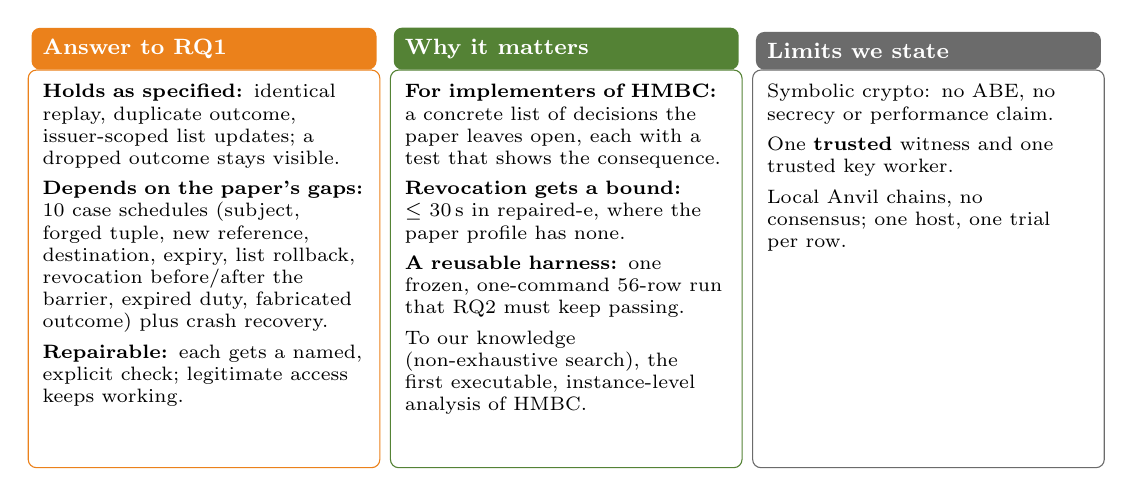
\begin{tikzpicture}[x=1cm, y=1cm, cw/.style={text width=4.1cm, draw=none, execute at begin node={\hyphenpenalty=10000\exhyphenpenalty=10000}}, hw/.style={text width=4.1cm, font=\footnotesize\bfseries}]
  \node[pcard=accent, cw] (k1) at (0,0) {%
    \textbf{Holds as specified:} identical replay, duplicate outcome, issuer-scoped list updates; a dropped outcome stays visible.\\[3pt]
    \textbf{Depends on the paper's gaps:} 10 case schedules (subject, forged tuple, new reference, destination, expiry, list rollback, revocation before/after the barrier, expired duty, fabricated outcome) plus crash recovery.\\[3pt]
    \textbf{Repairable:} each gets a named, explicit check; legitimate access keeps working.};
  \node[phead=accent, hw] at (0,0) {Answer to RQ1};
  \node[pcard=dbc, cw] (k2) at (4.6,0) {%
    \textbf{For implementers of HMBC:} a concrete list of decisions the paper leaves open, each with a test that shows the consequence.\\[3pt]
    \textbf{Revocation gets a bound:} $\le$ 30\,s in repaired-e, where the paper profile has none.\\[3pt]
    \textbf{A reusable harness:} one frozen, one-command 56-row run that RQ2 must keep passing.\\[3pt]
    To our knowledge (non-exhaustive search), the first executable, instance-level analysis of HMBC.};
  \node[phead=dbc, hw] at (4.6,0) {Why it matters};
  \node[pcard=datagray, cw] (k3) at (9.2,0) {%
    Symbolic crypto: no ABE, no secrecy or performance claim.\\[3pt]
    One \textbf{trusted} witness and one trusted key worker.\\[3pt]
    Local Anvil chains, no consensus; one host, one trial per row.};
  \node[phead=datagray, hw] at (9.2,0) {Limits we state};
  \foreach \k/\c in {1/accent, 2/dbc, 3/datagray} \draw[\c, rounded corners=3pt] (k\k.north west) rectangle ($(k\k.north east)+(0,-5.05)$);
\end{tikzpicture}

\vspace{0.5em}

\begin{tikzpicture}
  \node[draw=accent, fill=accent!10, rounded corners=3pt, text width=13.2cm, align=center, inner sep=5pt, font=\footnotesize]
    {Repaired-e puts all decision trust on \textbf{one witness}.\\RQ2 asks what survives when witnesses are Byzantine.};
\end{tikzpicture}
\end{frame}

% ================================================================ PART III: RQ2 (slides 15-27)
% Primary source: evaluation/reports/RQ2-F-DRAFT.md on origin/Code_Merge_Final (sha256 e59a51cd..) and the
% receipts it links under evaluation/evidence/f/. Nothing here is an integrated F case.

% ---------------------------------------------------------------- 15. RQ2 question and fault model
\begin{frame}{RQ2: what survives Byzantine witnesses?}
\begin{center}
\footnotesize\itshape Which RQ1 guarantees survive Byzantine operators with q-of-n application witnesses\\(n = 4, q = 3, f = 1), assuming safe ledgers and a trusted key worker?
\end{center}
\begin{columns}[T,onlytextwidth]
\column{0.50\textwidth}
\centering
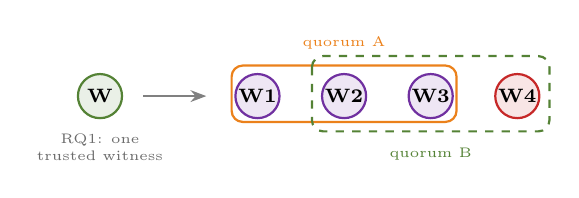
\begin{tikzpicture}[x=1cm, y=1cm]
  \node[wit=dbc] (e) at (0,0) {W};
  \node[font=\tiny, text=datagray, align=center, below=2pt of e] {RQ1: one\\trusted witness};
  \draw[->, thick, gray] (0.55,0) -- (1.35,0);
  \node[wit=pbc] (w1) at (2.0,0) {W1};
  \node[wit=pbc] (w2) at (3.1,0) {W2};
  \node[wit=pbc] (w3) at (4.2,0) {W3};
  \node[wit=badred] (w4) at (5.3,0) {W4};
  \draw[accent, thick, rounded corners] ($(w1.north west)+(-0.12,0.18)$) rectangle ($(w3.south east)+(0.12,-0.12)$);
  \draw[dbc, thick, dashed, rounded corners] ($(w2.north west)+(-0.2,0.3)$) rectangle ($(w4.south east)+(0.2,-0.24)$);
  \node[font=\tiny, text=accent, anchor=south] at ($(w1.north)!0.5!(w3.north)+(0,0.18)$) {quorum A};
  \node[font=\tiny, text=dbc, anchor=north] at ($(w2.south)!0.5!(w4.south)+(0,-0.24)$) {quorum B};
\end{tikzpicture}\\[0.3em]
\raggedright\scriptsize Any two 3-of-4 quorums share $\ge$ 2 witnesses, so with $f = 1$ they share an honest one. An honest witness never signs two conflicting decisions, so two conflicting certificates cannot both form.\\[0.4em]
\begin{alertblock}{Not a consensus protocol}
\scriptsize The witness layer authenticates decisions. It is not a new consensus, and Anvil is not Byzantine fault tolerant.
\end{alertblock}

\column{0.47\textwidth}
\footnotesize
\textbf{One witness per logical hospital.} Each checks the same accepted PBC decision and state \emph{itself}, then signs with its own off-chain key. The relay holds no witness key.\\[0.4em]
\textbf{Kept as stated assumptions, not proved}
\begin{itemize}\scriptsize\setlength{\itemsep}{1pt}
  \item safe ledgers: one local Anvil pair, no consensus;
  \item a trusted key worker: quorums do not remove it;
  \item eventual delivery, for progress.
\end{itemize}
\textbf{Deliberately outside the bound} (controls)
\begin{itemize}\scriptsize\setlength{\itemsep}{1pt}
  \item two Byzantine witnesses ($f = 2$);
  \item a weakened threshold ($q = 2$);
  \item a compromised quorum ($\ge$ 3 witnesses).
\end{itemize}
\end{columns}
\src{RQ2-F-DRAFT.md lines 127--132, 149, §3; SPEC.md §5}
\end{frame}

% ---------------------------------------------------------------- 16. RQ2 design
\begin{frame}{RQ2 design: three signed paths, governance, single-signing witnesses}
\begin{columns}[T,onlytextwidth]
\column{0.45\textwidth}
\centering
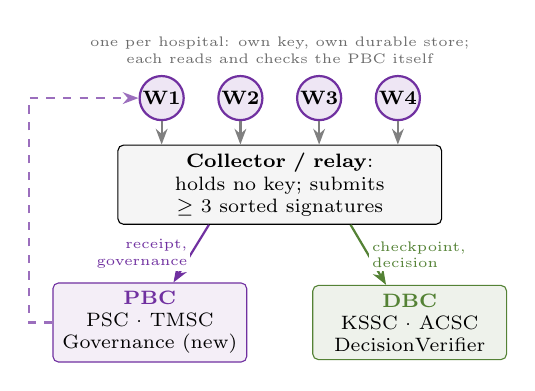
\begin{tikzpicture}[x=1cm, y=1cm]
  \foreach \i/\x in {1/1.5, 2/2.5, 3/3.5, 4/4.5} \node[wit=pbc] (w\i) at (\x,3.0) {W\i};
  \node[font=\tiny, text=datagray, anchor=south, align=center] at (3.0,3.32) {one per hospital: own key, own durable store;\\each reads and checks the PBC itself};
  \node[box, fill=gray!8, text width=3.9cm] (col) at (3.0,1.9) {\textbf{Collector / relay}: holds no key; submits $\ge$ 3 sorted signatures};
  \foreach \i in {1,...,4} \draw[->, gray, thick] (w\i.south) -- (w\i.south |- col.north);
  \node[box, draw=pbc, fill=pbc!8, text width=2.25cm] (pbc) at (1.35,0.15) {\textbf{\textcolor{pbc}{PBC}}\\PSC · TMSC\\Governance (new)};
  \node[box, draw=dbc, fill=dbc!10, text width=2.25cm] (dbc) at (4.65,0.15) {\textbf{\textcolor{dbc}{DBC}}\\KSSC · ACSC\\DecisionVerifier};
  \draw[->, thick, pbc] ($(col.south)+(-0.9,0)$) -- node[lbl, left, align=right, font=\tiny] {receipt,\\governance} ($(pbc.north)+(0.3,0)$);
  \draw[->, thick, dbc] ($(col.south)+(0.9,0)$) -- node[lbl, right, align=left, font=\tiny] {checkpoint,\\decision} ($(dbc.north)+(-0.3,0)$);
  \draw[->, dashed, thick, pbc!70] (pbc.west) -- ++(-0.3,0) |- (w1.west);
\end{tikzpicture}\\[0.4em]
\raggedright
\begin{itemize}\scriptsize\setlength{\itemsep}{1pt}
  \item \textbf{Governance:} add or remove a credential authority, set CA admins. A removed authority is tombstoned. The \textbf{witness set itself is fixed at deployment}.
\end{itemize}

\column{0.52\textwidth}
\scriptsize
\renewcommand{\arraystretch}{1.18}
\begin{tabular}{@{}L{0.19\linewidth} L{0.42\linewidth} L{0.33\linewidth}@{}}
\toprule
\textbf{Certificate} & \textbf{verified by} & \textbf{also rejected when} \\
\midrule
state checkpoint & {\ttfamily\fontsize{6}{7}\selectfont KSSC.acceptState} & sequence not strictly greater; auth epoch or source block lower \\
access decision & {\ttfamily\fontsize{6}{7}\selectfont ACSC.consumeDecision} & any of the 13 RQ1 checks fails \\
grant receipt & {\ttfamily\fontsize{6}{7}\selectfont PSC.reportAttestedOutcome} & it names another request, GID or record \\
governance action & {\ttfamily\fontsize{6}{7}\selectfont Governance.execute} & wrong nonce, or expired \\
\bottomrule
\end{tabular}

\vspace{0.4em}
\begin{itemize}\scriptsize\setlength{\itemsep}{1pt}
  \item Every path needs \textbf{$\ge$ q = 3 of the 4} member signatures, in strictly increasing signer order (4 of 4 is accepted).
  \item An honest witness \textbf{persists its one signature per decision key} before replying. After a grant has used the nonce, it refuses a fresh decision with \code{REPLAY}.
\end{itemize}
\end{columns}
\src{RQ2-F-DRAFT.md §1 (lines 127--132), §3 (line 269); A1-0137 §1 (SigLib.sol:37, Governance.sol:83--86, TMSC.sol:144--159), §2.1 (KSSC.sol:160--163); A2-0089 §2; SPEC.md §5}
\end{frame}

% ---------------------------------------------------------------- 17. How RQ2 will be judged
\begin{frame}{How RQ2 will be judged, and what exists today}
\begin{columns}[T,onlytextwidth]
\column{0.48\textwidth}
\footnotesize\textbf{The planned F gate: 32 cases in six families}\\[0.3em]
\scriptsize
\renewcommand{\arraystretch}{1.12}
\begin{tabular}{@{}L{0.72\linewidth} r@{}}
\toprule
\textbf{Family} & \textbf{cases} \\
\midrule
A\; quorum, availability, signature lists & 8 \\
B\; signing rule and Byzantine witness & 6 \\
C\; durable state, restart, tripwires & 4 \\
D\; trust lists and governance & 8 \\
E\; relay and outcomes & 3 \\
F\; compromise and residual inventory & 3 \\
\midrule
\textbf{integrated runs so far} & \textbf{0 of 32} \\
\bottomrule
\end{tabular}\\[0.4em]
Runner stages: 1--2 (pins, source bracket) implemented and fail closed (\code{BLOCKED}); 3--7 (owner baselines, family runs, verdicts, post bracket, manifest + E regression) in progress.\\[0.3em]
\src{plan-draft.json (families, stages; status DRAFT, authorizesExecution false); case-coverage-map-20261114}

\column{0.49\textwidth}
\footnotesize\textbf{Evidence collected so far (offline, synthetic fixtures)}\\[0.3em]
\scriptsize
\renewcommand{\arraystretch}{1.12}
\begin{tabular}{@{}L{0.78\linewidth} c@{}}
\toprule
\textbf{Evidence} & \textbf{label} \\
\midrule
TLC finite model, five configurations & \evl{F} \\
oracle/store differential + 7 mutations & \evl{U} \\
M5 Byzantine pool sweep & \evl{U} \\
M2 virtual availability sweep & \evl{U} \\
M6 real-process availability & \evl{R} \\
M1 gas and calldata & \evl{R} \\
K1 kill-durability test & \evl{R} \\
out-of-bound ledger tests & \evl{U} \\
\bottomrule
\end{tabular}\\[0.4em]
None of these is an F case. We measured what already existed, on purpose, before the runner and the FREEZE were ready.\\[0.2em]
\src{RQ2-F-DRAFT.md lines 3--10, §4; measurements-20261114/README.md lines 11--15}
\end{columns}
\end{frame}

% ---------------------------------------------------------------- 18. TLC
\begin{frame}{Safety 1: a finite model of one decision slot (TLC) \;\evl{F}}
\begin{columns}[T,onlytextwidth]
\column{0.60\textwidth}
\scriptsize
\renewcommand{\arraystretch}{1.3}
\begin{tabular}{@{}L{0.36\linewidth} L{0.22\linewidth} L{0.32\linewidth}@{}}
\toprule
\textbf{Configuration} & \textbf{role} & \textbf{Agreement} \\
\midrule
$f = 1$, $q = 3$, persistent single-signing & the claim & \textcolor{okgreen}{\textbf{holds}}: 433 states generated, 108 distinct, complete \\
$f = 0$, $q = 3$, persistent & positive control & \textcolor{okgreen}{\textbf{holds}}: 217 / 81, complete \\
$f = 1$, weak $q = 2$ & weakened mutant & \textcolor{badred}{\textbf{violated}} \\
$f = 2$, $q = 3$ & out-of-bound control & \textcolor{badred}{\textbf{violated}} (needs two Byzantine witnesses) \\
$f = 0$, honest witnesses may double-sign & no-persistence mutant & \textcolor{badred}{\textbf{violated}} \\
\bottomrule
\end{tabular}\\[0.4em]
\src{RQ2-F-DRAFT.md §2.1 (lines 141--158); tlc-audit-20261115/README.md lines 14--20}

\column{0.37\textwidth}
\footnotesize
\textbf{What it shows}
\begin{itemize}\scriptsize\setlength{\itemsep}{1pt}
  \item The quorum argument needs both halves: $q = 3$ \emph{and} honest witnesses that persist their one signature. Drop either, and TLC finds a violation.
  \item A fresh rerun on 15 Nov matched all five verdicts and state counts; agent 1's separate enumeration matches the complete counts.
\end{itemize}
\textbf{What it does not}
\begin{itemize}\scriptsize\setlength{\itemsep}{1pt}
  \item One slot, a fixed witness set: no expiry, checkpoint advance or superseded pins.
  \item Not a proof of the implementation, of consensus or of liveness.
\end{itemize}
\scriptsize\color{datagray} Our first $f = 0$ run deadlocked (a model error of ours); it is kept in the record.
\end{columns}
\end{frame}

% ---------------------------------------------------------------- 19. Oracle/store differential + mutations
\begin{frame}{Safety 2: does our oracle agree with the witness store? \;\evl{U}}
\begin{columns}[T,onlytextwidth]
\column{0.40\textwidth}
\footnotesize
\scriptsize
The evaluator's fault oracle (independent rules) and agent 2's durable \code{WitnessStore} (SQLite) decide the same 180 synthetic signing requests, across the four signing kinds.\\[0.5em]
\centering
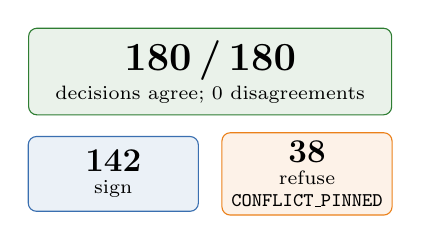
\begin{tikzpicture}[x=1cm, y=1cm, every node/.append style={font=\scriptsize}]
  \node[tile=okgreen, text width=4.4cm, minimum height=1.1cm] at (0,0) {{\Large\bfseries 180 / 180}\\[1pt]decisions agree; 0 disagreements};
  \node[tile=clsup, text width=1.95cm, minimum height=0.95cm] at (-1.23,-1.3) {{\large\bfseries 142}\\sign};
  \node[tile=accent, text width=1.95cm, minimum height=0.95cm] at (1.23,-1.3) {{\large\bfseries 38}\\refuse \code{CONFLICT\_PINNED}};
\end{tikzpicture}\\[0.3em]
\raggedright\scriptsize Rerun on 15 Nov against the adopted protocol source (subtree \code{7566f63d..}).

\column{0.57\textwidth}
\centering
\footnotesize\textbf{Seven deliberate oracle bugs: each one is caught}\\[0.1em]
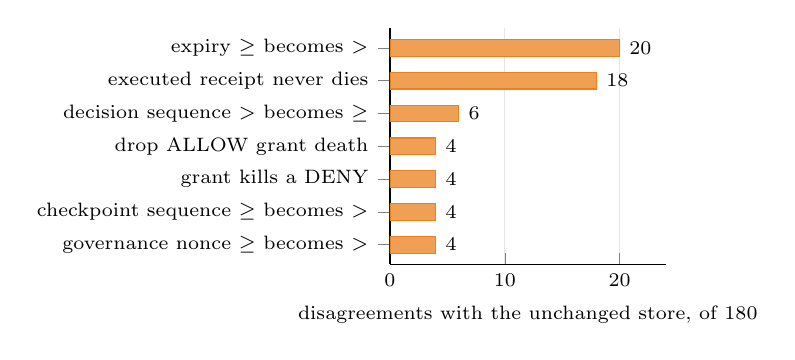
\begin{tikzpicture}
\begin{axis}[
    xbar, bar width=6pt, scale only axis, width=3.5cm, height=3.0cm,
    xmin=0, xmax=24, axis x line*=bottom, axis y line*=left,
    ytick={1,...,7}, y dir=reverse,
    yticklabels={{expiry $\ge$ becomes $>$}, {executed receipt never dies}, {decision sequence $>$ becomes $\ge$}, {drop ALLOW grant death}, {grant kills a DENY}, {checkpoint sequence $\ge$ becomes $>$}, {governance nonce $\ge$ becomes $>$}},
    tick label style={font=\scriptsize}, xlabel style={font=\scriptsize},
    xlabel={disagreements with the unchanged store, of 180},
    nodes near coords, nodes near coords style={font=\scriptsize},
    enlarge y limits=0.1, xmajorgrids, grid style={gray!20},
  ]
  \addplot[fill=accent!75, draw=accent] coordinates {(20,1) (18,2) (6,3) (4,4) (4,5) (4,6) (4,7)};
\end{axis}
\end{tikzpicture}\\[0.2em]
\raggedright\scriptsize Baseline stays 180/180; all seven counts reproduce the 14 Nov receipt.
\end{columns}

\vspace{0.2em}
\begin{alertblock}{Scope}
\scriptsize Sensitivity to these seven rule errors, not completeness of the oracle. It tests what the \emph{store} can do, not what the service or the ledger lets happen. Our earlier claim that an honest DENY can follow a used ALLOW was wrong and is corrected: the honest service answers \code{REPLAY} first (confirmed by agent 2).
\end{alertblock}
\src{oracle-store-diff-20261115/README.md lines 9--16; oracle-mutant-discrimination-20261115/README.md lines 9--24; RQ2-F-DRAFT.md lines 293--301; A2-0089 §2}
\end{frame}

% ---------------------------------------------------------------- 20. M5 pool sweep
\begin{frame}{Safety 3: a Byzantine sweep over the real witness pool (M5) \;\evl{U}}
\begin{columns}[T,onlytextwidth]
\column{0.55\textwidth}
\centering
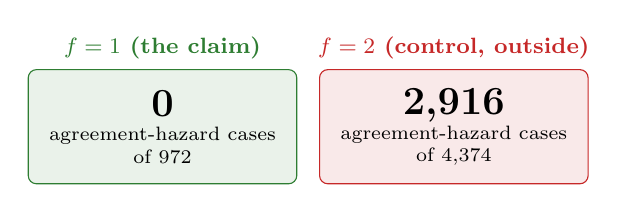
\begin{tikzpicture}[x=1cm, y=1cm, every node/.append style={font=\scriptsize}]
  \node[font=\footnotesize\bfseries, text=okgreen] at (-1.85,1.15) {$f = 1$ (the claim)};
  \node[font=\footnotesize\bfseries, text=badred] at (1.85,1.15) {$f = 2$ (control, outside)};
  \node[tile=okgreen, text width=3.2cm, minimum height=1.45cm] at (-1.85,0.15) {{\Large\bfseries 0}\\[1pt]agreement-hazard cases\\of 972};
  \node[tile=badred, text width=3.2cm, minimum height=1.45cm] at (1.85,0.15) {{\Large\bfseries 2,916}\\[1pt]agreement-hazard cases\\of 4,374};
\end{tikzpicture}\\[0.5em]
\scriptsize
\renewcommand{\arraystretch}{1.18}
\begin{tabular}{@{}l r r r r@{}}
\toprule
Bound & cases & certificates & no certificate & invalid certificates \\
\midrule
$f = 1$ & 972 & 180 & 792 & 0 \\
$f = 2$ & 4,374 & 330 & 4,044 & 0 \\
\bottomrule
\end{tabular}\\[0.3em]
\raggedright\scriptsize Every accepted certificate has 3 distinct, sorted, valid signers. ``No certificate'' comes from honest pin splits: unavailable, not unsafe.

\column{0.42\textwidth}
\footnotesize
\textbf{Setup}
\begin{itemize}\scriptsize\setlength{\itemsep}{1pt}
  \item Agent 2's pool state machine, real EIP-712 signatures.
  \item 9 Byzantine behaviours: silent; a valid signature over value A, B or C; a recorded report over A, B or C; garbage; a wrong-key signature.
  \item $f = 1$: 4 positions $\times$ 9 behaviours $\times$ 27 honest pin patterns.
  \item $f = 2$: 6 position pairs $\times$ 81 behaviour pairs $\times$ 9 pin patterns.
\end{itemize}
\textbf{Hazard} (our definition): after the run, two different values could each gather $\ge$ 3 signers. A \emph{potential} conflict, not two realised certificates.\\[0.3em]
\textbf{Limits:} honest witnesses are a model of the signing rule, not the durable store; virtual transport. Rerun on 15 Nov from the exact source: byte-identical output.
\end{columns}
\src{pool-sweep-20261115/README.md lines 15--30; measurements-20261114/README.md lines 69--83; RQ2-F-DRAFT.md §2.2}
\end{frame}

% ---------------------------------------------------------------- 21. Availability
\begin{frame}{Availability: one witness down still certifies; two do not}
\begin{columns}[T,onlytextwidth]
\column{0.47\textwidth}
\footnotesize\textbf{M2: all 16 muted subsets, 5 runs each (virtual time)} \evl{U}\\[0.5em]
\centering
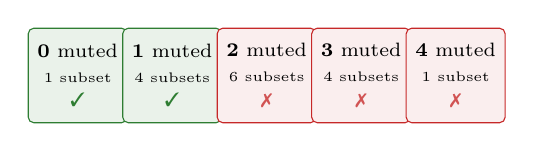
\begin{tikzpicture}[x=1cm, y=1cm, c/.style={draw, rounded corners=2pt, minimum width=1.05cm, minimum height=1.2cm, align=center, font=\scriptsize}]
  \foreach \i/\n/\ok in {0/1/1, 1/4/1, 2/6/0, 3/4/0, 4/1/0} {
    \ifnum\ok=1
      \node[c, draw=okgreen, fill=okgreen!10] at (\i*1.2,0) {\textbf{\i} muted\\[1pt]{\tiny \n{} subset\ifnum\n>1 s\fi}\\[1pt]\cmark};
    \else
      \node[c, draw=badred, fill=badred!8] at (\i*1.2,0) {\textbf{\i} muted\\[1pt]{\tiny \n{} subset\ifnum\n>1 s\fi}\\[1pt]\xmark};
    \fi
  }
\end{tikzpicture}\\[0.4em]
\raggedright\scriptsize
\cmark\ a 3-signature certificate in every run \quad \xmark\ none by the 10\,s deadline\\[0.3em]
Replies delayed 400 / 300 / 200 / 100\,ms: the certificate forms from the three fastest at 300\,ms; the slowest witness is not waited for.\\[0.3em]
Four real witnesses (durable SQLite stores, real signatures) behind a virtual transport; rerun on 15 Nov on the exact source: all 80 trials match.

\column{0.50\textwidth}
\footnotesize\textbf{M6: real processes, local Anvil pair, real KSSC} \evl{R}\\[0.4em]
\scriptsize
\renewcommand{\arraystretch}{1.25}
\begin{tabular}{@{}L{0.50\linewidth} r r r@{}}
\toprule
\textbf{Scenario (test-body time)} & \textbf{run 1} & \textbf{run 2} & \textbf{run 3} \\
\midrule
4 live witnesses, q = 3 certificate accepted & 0.69\,s & 0.69\,s & 0.78\,s \\
1 witness SIGKILLed: 3 signers, accepted & 0.63\,s & 0.55\,s & 0.60\,s \\
2 witnesses stopped: classified timeout & 10.54\,s & 10.54\,s & 10.55\,s \\
killed witness restarted keeps its durable pin & 0.96\,s & 0.87\,s & 0.88\,s \\
\bottomrule
\end{tabular}\\[0.4em]
Agent 2's live tests, run unmodified on the evaluator's host: 4 passed in each of three runs. The 10.5\,s is the pool's 10\,s deadline plus overhead.\\[0.3em]
\scriptsize\color{datagray} The raw stdout and exact invocation of these three runs were not retained: they are prior reported runs. No network, no block time, one host. No liveness claim under arbitrary delay.
\end{columns}
\src{measurements-20261114/README.md lines 41--52, 118--134; availability-reproduction-20261115; availability-receipt-review-20261115/README.md lines 1--6; RQ2-F-DRAFT.md §2.3}
\end{frame}

% ---------------------------------------------------------------- 22. Gas
\begin{frame}{Cost: what three signatures cost on chain (M1, M1b, M1c) \;\evl{R}}
\begin{columns}[T,onlytextwidth]
\column{0.55\textwidth}
\centering
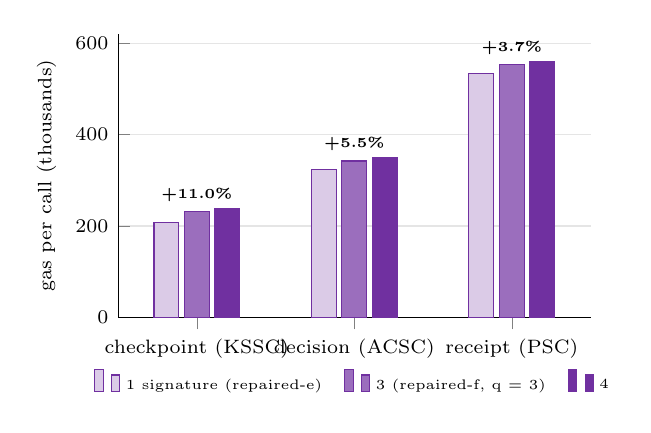
\begin{tikzpicture}
\begin{axis}[
    ybar, bar width=9pt, scale only axis, width=6.0cm, height=3.6cm,
    ymin=0, ymax=620, axis x line*=bottom, axis y line*=left,
    symbolic x coords={checkpoint,decision,receipt},
    xtick=data, enlarge x limits=0.25,
    xticklabels={{checkpoint (KSSC)}, {decision (ACSC)}, {receipt (PSC)}},
    xticklabel style={font=\scriptsize},
    ylabel={gas per call (thousands)}, ylabel style={font=\scriptsize},
    yticklabel style={font=\scriptsize},
    ymajorgrids, grid style={gray!20},
    legend style={font=\tiny, at={(0.5,-0.16)}, anchor=north, draw=none, fill=white, legend columns=3, /tikz/every even column/.append style={column sep=6pt}},
    legend cell align=left,
  ]
  \addplot[fill=pbc!25, draw=pbc] coordinates {(checkpoint,208.290) (decision,324.323) (receipt,533.754)};
  \addplot[fill=pbc!70, draw=pbc, nodes near coords, point meta=explicit symbolic, nodes near coords style={font=\tiny\bfseries, text=black}]
    coordinates {(checkpoint,231.260)[+11.0\%] (decision,342.261)[+5.5\%] (receipt,553.488)[+3.7\%]};
  \addplot[fill=pbc, draw=pbc] coordinates {(checkpoint,238.046) (decision,349.053) (receipt,560.290)};
  \legend{{1 signature (repaired-e)}, {3 (repaired-f, q = 3)}, {4}}
\end{axis}
\end{tikzpicture}\\
\src{Forge 1.8.5 gas of one external call; same F commit, E profile vs F profile}

\column{0.42\textwidth}
\scriptsize
\renewcommand{\arraystretch}{1.2}
\begin{tabular}{@{}l r r r@{}}
\toprule
\textbf{call} & \textbf{1 sig} & \textbf{3 sigs} & \textbf{4 sigs} \\
\midrule
checkpoint & 208,290 & 231,260 & 238,046 \\
decision & 324,323 & 342,261 & 349,053 \\
receipt & 533,754 & 553,488 & 560,290 \\
\bottomrule
\end{tabular}\\[0.4em]
\begin{itemize}\scriptsize\setlength{\itemsep}{1pt}
  \item Each extra signature: $\approx$ 6.8k gas and 160 bytes of calldata.
  \item \code{Governance.execute} (F only, 3 signatures): add authority 524,214; remove 424,421; set CA admins 446,934.
  \item All product contracts stay under the 24,576\,B limit; TMSC grew from 12,635\,B (E-era) to 16,127\,B.
  \item Measured by the evaluator; agent 1 reproduced all 21 emitted rows (15 distinct) exactly, raw logs retained.
\end{itemize}
\scriptsize\color{datagray} Single deterministic runs; not a fee estimate. A cold-storage explanation of the fixed F overhead was tested and refuted (231,261 vs 231,260 gas).
\end{columns}
\src{measurements-20261114/README.md lines 23--39, 85--111; RQ2-F-DRAFT.md §2.4; A1-0123, A1-0124, A1-0125, A1-0136}
\end{frame}

% ---------------------------------------------------------------- 23. K1
\begin{frame}{Durability: making a kill test deterministic (K1) \;\evl{R}}
\begin{columns}[T,onlytextwidth]
\column{0.37\textwidth}
\footnotesize\textbf{The mutant K1}\\[0.3em]
\centering
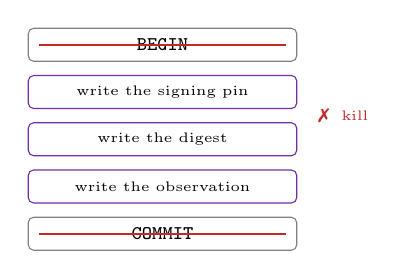
\begin{tikzpicture}[x=1cm, y=1cm, st/.style={box, text width=3.2cm, minimum height=0.42cm, fill=white, font=\tiny}]
  \node[st, draw=gray] (b) at (0,0) {\code{BEGIN}};
  \node[st, draw=pbc] (p) at (0,-0.6) {write the signing pin};
  \node[st, draw=pbc] (d) at (0,-1.2) {write the digest};
  \node[st, draw=pbc] (o) at (0,-1.8) {write the observation};
  \node[st, draw=gray] (c) at (0,-2.4) {\code{COMMIT}};
  \draw[badred, thick] ($(b.west)+(0.15,0)$) -- ($(b.east)+(-0.15,0)$);
  \draw[badred, thick] ($(c.west)+(0.15,0)$) -- ($(c.east)+(-0.15,0)$);
  \node[text=badred, font=\scriptsize\bfseries] at (2.05,-0.9) {\ding{55}};
  \node[font=\tiny, text=badred, anchor=west] at (2.15,-0.9) {kill};
\end{tikzpicture}\\[0.3em]
\raggedright\scriptsize K1 removes the signing transaction, so each write commits alone. A kill between two writes leaves a pin without its digest: a torn record that the test must catch.

\column{0.30\textwidth}
\centering
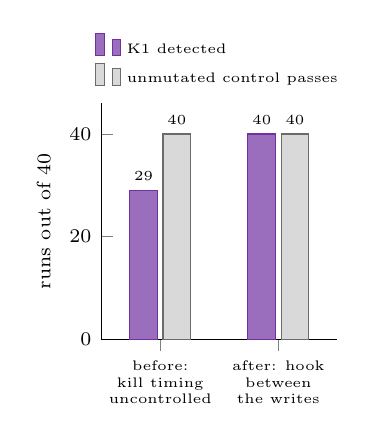
\begin{tikzpicture}
\begin{axis}[
    ybar, bar width=10pt, scale only axis, width=3.0cm, height=3.0cm,
    ymin=0, ymax=46, axis x line*=bottom, axis y line*=left,
    symbolic x coords={before,after}, xtick=data, enlarge x limits=0.5,
    xticklabels={{before:\\kill timing\\uncontrolled}, {after: hook\\between\\the writes}},
    xticklabel style={align=center, font=\tiny},
    ylabel={runs out of 40}, ylabel style={font=\scriptsize}, yticklabel style={font=\scriptsize},
    nodes near coords, nodes near coords style={font=\tiny},
    legend style={font=\tiny, at={(0.5,1.02)}, anchor=south, draw=none, legend columns=1},
    legend cell align=left,
  ]
  \addplot[fill=pbc!70, draw=pbc] coordinates {(before,29) (after,40)};
  \addplot[fill=gray!30, draw=datagray] coordinates {(before,40) (after,40)};
  \legend{K1 detected, unmutated control passes}
\end{axis}
\end{tikzpicture}

\column{0.31\textwidth}
\scriptsize
\begin{itemize}\setlength{\itemsep}{2pt}
  \item The earlier ``K1 detected 3 of 3'' did not reproduce: we measured \textbf{29 of 40} (72.5\%).
  \item Fix: a test hook \emph{between} the signing writes. Then \textbf{40 of 40} detected, controls 40 of 40.
  \item Agent 2's own rerun: 15 of 15 detected, 10 of 10 controls, 81 state tests; full protocol suite 3,226 passed, 201 skipped.
  \item The same review also found and fixed: a store refused after a kill during init; a snapshot-lock defect; an anchor-selection bug in our evaluator.
\end{itemize}
\end{columns}

\vspace{0.4em}
{\scriptsize\textbf{\textcolor{accent}{Scope:}} SIGKILL only. The mutant that turns off \code{synchronous=FULL} survives, because only power loss could show it: no power-loss claim, and no production corruption rate.}\\[0.1em]
\src{reviews/a2-0086-signing-kill-20261113/README.md lines 14--36; reviews/proxy-k1-20261114/README.md lines 46--55; A2-0089 §1; protocol/tools/run\_state\_kill\_mutants.py lines 5--9; RQ2-F-DRAFT.md §2.5}
\end{frame}

% ---------------------------------------------------------------- 24. Trust matrix
\begin{frame}{The trust matrix: what RQ2 still has to trust}
\scriptsize
\renewcommand{\arraystretch}{1.17}
\begin{tabular}{@{}L{0.27\textwidth} c L{0.53\textwidth}@{}}
\toprule
\textbf{Component} & \textbf{status} & \textbf{What that means} \\
\midrule
$\ge$ 3 of 4 witnesses honest & \stt{accent}{REQUIRED} & the $f = 1$ bound; also no shared source-view failure \\
governance quorum & \stt{accent}{REQUIRED} & a compromised quorum ($\ge$ 3) can halt a DBC or grant to a fabricated requester (next slide) \\
key worker and its host & \stt{datagray}{TRUSTED} & quorums do not stop a compromised worker using its own keys; that F case is NOT\_RUN \\
credential authority & \stt{datagray}{TRUSTED} & trusted for what it issues; a quorum does not make a credential true \\
relay / collector & \stt{clsup}{NO KEY} & cannot forge; can withhold or delay, so progress needs eventual delivery \\
the local Anvil pair & \stt{datagray}{ASSUMED} & assumed correct; consensus not evaluated \\
witness processes & \stt{clsup}{SEPARATE} & own stores, keys and processes, but one host: no independence from a shared OS or operator \\
durable witness store & \stt{clsup}{TESTED} & SIGKILL only; no power-loss claim \\
key custody & \stt{badred}{NOT EVALUATED} & TEST-ONLY synthetic keys \\
client and data store & \stt{badred}{NOT EVALUATED} & retention, availability and real confidentiality are not established by F \\
authors of code and reviews & \stt{badred}{CORRELATED} & one model family wrote and reviewed everything \\
\bottomrule
\end{tabular}

\vspace{0.4em}
\src{RQ2-F-DRAFT.md §3 (lines 265--278); SPEC.md §5 (the trust matrix must cover ledgers, relay, witness keys, authority, key worker, client and store)}
\end{frame}

% ---------------------------------------------------------------- 25. Outside the bound
\begin{frame}{Outside the bound: what too many Byzantine witnesses can do}
\centering
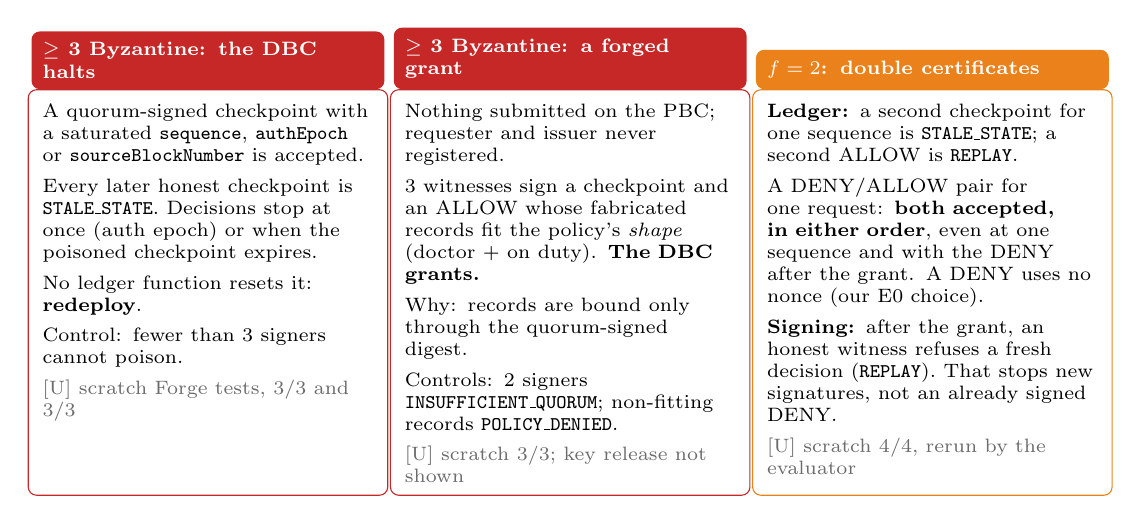
\begin{tikzpicture}[x=1cm, y=1cm, cw/.style={text width=4.2cm, draw=none, execute at begin node={\hyphenpenalty=10000\exhyphenpenalty=10000}}, hw/.style={text width=4.2cm, font=\scriptsize\bfseries}]
  \node[pcard=badred, cw] (k1) at (0,0) {%
    A quorum-signed checkpoint with a saturated \code{sequence}, \code{authEpoch} or \code{sourceBlockNumber} is accepted.\\[3pt]
    Every later honest checkpoint is \code{STALE\_STATE}. Decisions stop at once (auth epoch) or when the poisoned checkpoint expires.\\[3pt]
    No ledger function resets it: \textbf{redeploy}.\\[3pt]
    Control: fewer than 3 signers cannot poison.\\[3pt]
    {\color{datagray}[U] scratch Forge tests, 3/3 and 3/3}};
  \node[phead=badred, hw] at (0,0) {$\ge$ 3 Byzantine: the DBC halts};
  \node[pcard=badred, cw] (k2) at (4.6,0) {%
    Nothing submitted on the PBC; requester and issuer never registered.\\[3pt]
    3 witnesses sign a checkpoint and an ALLOW whose fabricated records fit the policy's \emph{shape} (doctor + on duty). \textbf{The DBC grants.}\\[3pt]
    Why: records are bound only through the quorum-signed digest.\\[3pt]
    Controls: 2 signers \code{INSUFFICIENT\_QUORUM}; non-fitting records \code{POLICY\_DENIED}.\\[3pt]
    {\color{datagray}[U] scratch 3/3; key release not shown}};
  \node[phead=badred, hw] at (4.6,0) {$\ge$ 3 Byzantine: a forged grant};
  \node[pcard=accent, cw] (k3) at (9.2,0) {%
    \textbf{Ledger:} a second checkpoint for one sequence is \code{STALE\_STATE}; a second ALLOW is \code{REPLAY}.\\[3pt]
    A DENY/ALLOW pair for one request: \textbf{both accepted, in either order}, even at one sequence and with the DENY after the grant. A DENY uses no nonce (our E0 choice).\\[3pt]
    \textbf{Signing:} after the grant, an honest witness refuses a fresh decision (\code{REPLAY}). That stops new signatures, not an already signed DENY.\\[3pt]
    {\color{datagray}[U] scratch 4/4, rerun by the evaluator}};
  \node[phead=accent, hw] at (9.2,0) {$f = 2$: double certificates};
  \foreach \k/\c in {1/badred, 2/badred, 3/accent} \draw[\c, rounded corners=3pt] (k\k.north west) rectangle ($(k\k.north east)+(0,-5.15)$);
\end{tikzpicture}

\vspace{0.1em}
\scriptsize These need a compromised quorum or two Byzantine witnesses: they do \textbf{not} contradict the $f \le 1$ claims. Tested reconstruction results, not HMBC vulnerabilities.\\[0.1em]
\src{RQ2-F-DRAFT.md §3 (lines 269, 279--291); A1-0137 §2; A1-0138 §1--2; A1-0141 §2--3; A1-0126 / measurements-20261114 line 141--144}
\end{frame}

% ---------------------------------------------------------------- 26. Assurance process
\begin{frame}{Assurance: how the evidence was checked, and what we got wrong}
\begin{columns}[T,onlytextwidth]
\column{0.45\textwidth}
\footnotesize\textbf{Exact-hash, scoped reviews}
\begin{itemize}\scriptsize\setlength{\itemsep}{2pt}
  \item The partial RQ2 report is pinned by SHA-256 (\code{e59a51cd..}). The ledger role (A1-0142) and protocol role (A2-0091) each read the full diff and found no objection \emph{in their scope}.
  \item Excluded: evaluation-tool correctness. A review is not an execution ACK and does not cover any later revision.
  \item Every receipt records commands, exit codes, source pins and output hashes; peers re-run where they can (gas, K1, TLC counts).
\end{itemize}
\begin{alertblock}{Correlated, not independent}
\scriptsize All three roles are the same model family. These are scoped re-checks, not independent review.
\end{alertblock}

\column{0.52\textwidth}
\footnotesize\textbf{Errors caught, and kept in the record}\\[0.2em]
\scriptsize
\renewcommand{\arraystretch}{1.18}
\begin{tabular}{@{}L{0.47\linewidth} L{0.47\linewidth}@{}}
\toprule
\textbf{Claimed} & \textbf{Corrected to} \\
\midrule
an honest DENY can follow a used ALLOW & wrong: the honest service says \code{REPLAY} first \\
report §3 mixed ledger acceptance with honest signing & split into two statements (A1-0141) \\
M1 gas test count 9/9 & 6/6 (A1-0136) \\
ledger plan checker 27/27 & its dev-key scan read a missing directory; now 28/28 + 9/9 negative controls \\
TMSC size 52,339\,B & a parser artifact; real size 16,127\,B \\
K1 detected 3/3 & 29/40; then fixed to 40/40 \\
a report section was ``byte-identical'' & only its first line was hashed; now whole paragraphs \\
\bottomrule
\end{tabular}
\end{columns}
\src{BOARD.md A3-0160; partial-report-packet-20261115/README.md lines 3--43; RQ2-F-DRAFT.md lines 49--55, 216--217, 293--301; A1-0136 §2; A1-0141 §5}
\end{frame}

% ================================================================ PART IV: status, limits, conclusion (slides 27-30)

% ---------------------------------------------------------------- 27. Honest status
\begin{frame}{Honest status of RQ2 on 17 November}
\centering
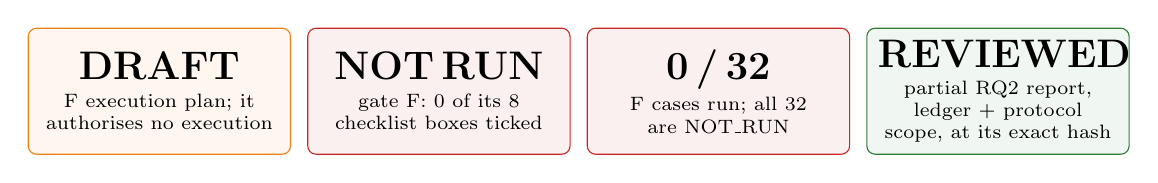
\begin{tikzpicture}[x=1cm, y=1cm, every node/.append style={minimum height=1.55cm, font=\scriptsize, execute at begin node={\hyphenpenalty=10000\exhyphenpenalty=10000}}]
  \node[stat=accent]   at (0,0)     {{\Large\bfseries DRAFT}\\[2pt]F execution plan; it authorises no execution};
  \node[stat=badred]   at (3.55,0)  {{\Large\bfseries NOT RUN}\\[2pt]gate F: 0 of its 8 checklist boxes ticked};
  \node[stat=badred]   at (7.1,0)   {{\Large\bfseries 0 / 32}\\[2pt]F cases run; all 32 are NOT\_RUN};
  \node[stat=okgreen]  at (10.65,0) {{\Large\bfseries REVIEWED}\\[2pt]partial RQ2 report, ledger + protocol scope, at its exact hash};
\end{tikzpicture}

\vspace{0.5em}
\begin{columns}[T,onlytextwidth]
\column{0.49\textwidth}
\footnotesize\textbf{Done (offline)}
\begin{itemize}\scriptsize\setlength{\itemsep}{1pt}
  \item F0 fault model accepted by all roles (4 Nov); ledger and protocol code built and owner-tested.
  \item Partial RQ2 report, reviewed in ledger and protocol scope at its exact hash (16 Nov).
  \item Runner stages 1--2; parts of stage 3 (baseline executor, snapshot materialiser, witness-RPC capture), tested on synthetic inputs.
  \item Merged snapshot \code{Code\_Merge\_Final}: ledger 316 passed; protocol 3,226 passed, 201 skipped; evaluation 3,097 passed, 4 failed (host-specific; the same 4 on the agent-3 tip).
\end{itemize}

\column{0.48\textwidth}
\footnotesize\textbf{Still needed before gate F}
\begin{enumerate}\scriptsize\setlength{\itemsep}{1pt}
  \item an exact execution FREEZE, with the ACK of each role on that plan hash;
  \item runner stages 3--7 finished, including authenticated, complete signer capture;
  \item the 32 integrated cases, positive controls first;
  \item RQ1's suites re-run on the F ledger (E regression);
  \item \code{RQ2-F.md}, then three matching sign-offs.
\end{enumerate}
\end{columns}
\src{plan-draft.json; GATES.md lines 650--661; BOARD.md A3-0161, A3-0162, A3-0163; partial-report-packet-20261115/README.md lines 124--141; A1-0145 §2 (origin/agent-1)}
\end{frame}

% ---------------------------------------------------------------- 28. Limitations and lessons
\begin{frame}{Limitations and lessons}
\begin{columns}[T,onlytextwidth]
\column{0.48\textwidth}
\footnotesize\textbf{Limitations}
\begin{itemize}\scriptsize\setlength{\itemsep}{1pt}
  \item \textbf{Correlated review:} one model family wrote and reviewed every module.
  \item \textbf{Synthetic fixtures:} TEST-ONLY keys, one fixed policy, one host, local Anvil.
  \item \textbf{Model $\neq$ implementation:} TLC checks one decision slot; ProVerif is symbolic.
  \item \textbf{Offline $\neq$ integrated:} no RQ2 number is an F case yet.
  \item \textbf{Symbolic crypto:} no ABE, so no secrecy or performance claim.
\end{itemize}
\textbf{What F does not prove, even when it passes}
\begin{itemize}\scriptsize\setlength{\itemsep}{1pt}
  \item consensus, or safety with $\ge$ 2 Byzantine witnesses;
  \item liveness under arbitrary delay, or real-network latency;
  \item power-loss durability, or protection from a compromised key worker.
\end{itemize}

\column{0.49\textwidth}
\footnotesize\textbf{Lessons}
\begin{enumerate}\scriptsize\setlength{\itemsep}{3pt}
  \item \textbf{A random fault point can look green.} K1 was reported detected 3 of 3; in 40 runs we saw 29. Put the fault point where the bug lives.
  \item \textbf{Check your checks for vacuity.} A secret scan of a missing directory ``passes''.
  \item \textbf{Bind by value, not by label.} The $q = 2$ mutant's manifest says \code{repaired-f}; only the threshold (2 vs.\ 3, read back on chain) tells them apart.
  \item \textbf{Hash the whole artifact.} A first-line hash missed an edited sentence.
  \item \textbf{Keep signing rules and ledger rules apart.} An honest witness's \code{REPLAY} does not stop an already signed DENY.
\end{enumerate}
\end{columns}
\src{RQ2-F-DRAFT.md §5; RQ1-E.md §15; A1-0143 §2.1; A1-0141 §5; RQ2-F-DRAFT.md lines 49--55}
\end{frame}

% ---------------------------------------------------------------- 29. Conclusion
\begin{frame}{Conclusion}
\centering
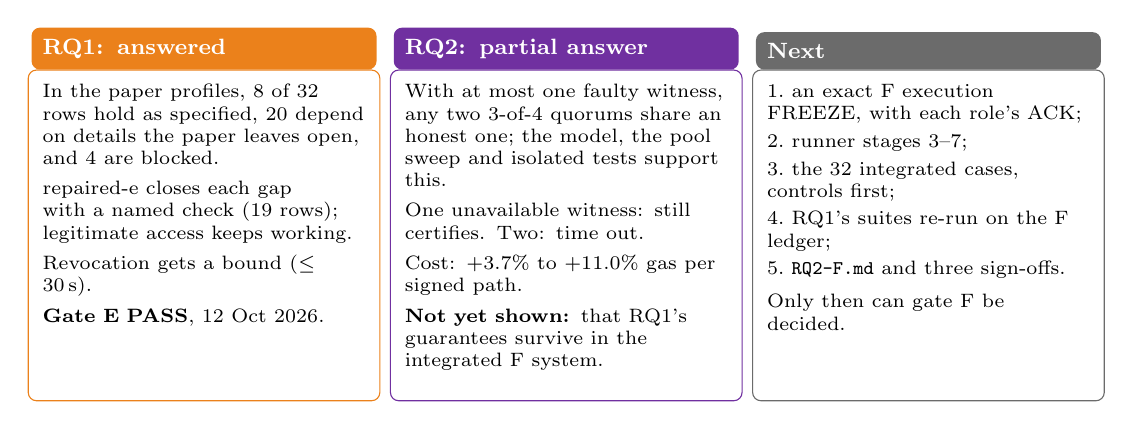
\begin{tikzpicture}[x=1cm, y=1cm, cw/.style={text width=4.1cm, draw=none, execute at begin node={\hyphenpenalty=10000\exhyphenpenalty=10000}}, hw/.style={text width=4.1cm, font=\footnotesize\bfseries}]
  \node[pcard=accent, cw] (k1) at (0,0) {%
    In the paper profiles, 8 of 32 rows hold as specified, 20 depend on details the paper leaves open, and 4 are blocked.\\[3pt]
    repaired-e closes each gap with a named check (19 rows); legitimate access keeps working.\\[3pt]
    Revocation gets a bound ($\le$ 30\,s).\\[3pt]
    \textbf{Gate E PASS}, 12 Oct 2026.};
  \node[phead=accent, hw] at (0,0) {RQ1: answered};
  \node[pcard=pbc, cw] (k2) at (4.6,0) {%
    With at most one faulty witness, any two 3-of-4 quorums share an honest one; the model, the pool sweep and isolated tests support this.\\[3pt]
    One unavailable witness: still certifies. Two: time out.\\[3pt]
    Cost: +3.7\% to +11.0\% gas per signed path.\\[3pt]
    \textbf{Not yet shown:} that RQ1's guarantees survive in the integrated F system.};
  \node[phead=pbc, hw] at (4.6,0) {RQ2: partial answer};
  \node[pcard=datagray, cw] (k3) at (9.2,0) {%
    1.\ an exact F execution FREEZE, with each role's ACK;\\[2pt]
    2.\ runner stages 3--7;\\[2pt]
    3.\ the 32 integrated cases, controls first;\\[2pt]
    4.\ RQ1's suites re-run on the F ledger;\\[2pt]
    5.\ \code{RQ2-F.md} and three sign-offs.\\[4pt]
    Only then can gate F be decided.};
  \node[phead=datagray, hw] at (9.2,0) {Next};
  \foreach \k/\c in {1/accent, 2/pbc, 3/datagray} \draw[\c, rounded corners=3pt] (k\k.north west) rectangle ($(k\k.north east)+(0,-4.2)$);
\end{tikzpicture}

\vspace{0.3em}
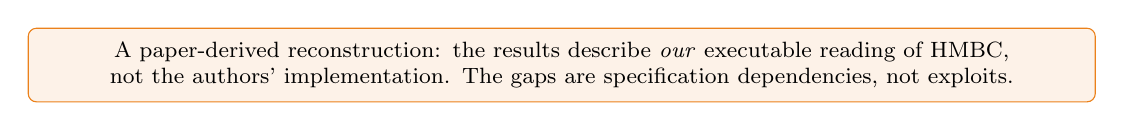
\begin{tikzpicture}
  \node[draw=accent, fill=accent!10, rounded corners=3pt, text width=13.2cm, align=center, inner sep=5pt, font=\footnotesize]
    {A paper-derived reconstruction: the results describe \emph{our} executable reading of HMBC,\\not the authors' implementation. The gaps are specification dependencies, not exploits.};
\end{tikzpicture}
\src{RQ1-E.md §0, §6; RQ2-F-DRAFT.md lines 19--24, §2.3, §2.4; GATES.md lines 650--661; packet README lines 131--141}
\end{frame}

% ---------------------------------------------------------------- 30. Close
\begin{frame}[standout]
Thank you\\[0.5em]
{\normalsize Questions?}
\end{frame}

\end{document}